\documentclass[13pt,a4paper]{extarticle}
\usepackage[utf8]{inputenc}
\usepackage[T5]{fontenc}
\usepackage[vietnamese]{babel}
\usepackage{mathptmx} % Phông chữ Times New Roman cho văn bản và công thức toán
\usepackage{geometry}
\geometry{top=2.5cm, bottom=2.5cm, left=3.0cm, right=2.0cm} % Chuẩn luận văn: lề trái 3cm đóng gáy
\usepackage{setspace}
\setstretch{1.3} % Giãn dòng 1.3 chuẩn văn bản học thuật
\usepackage{graphicx}
\graphicspath{{figures/}{../outputs/figures/}{./}}
\usepackage{booktabs}
\usepackage{array}
\usepackage{float}
\usepackage{amsmath}
\usepackage{amssymb}
\usepackage[unicode]{hyperref}
\usepackage{listings}
\usepackage{xcolor}
\usepackage{tikz}
\usetikzlibrary{calc}
\usepackage{titlesec}
\usepackage{enumitem}

% Cấu hình tiêu đề theo đúng yêu cầu: Tiêu đề lớn cỡ 16pt, tiểu mục 14pt, nội dung 13pt
\titleformat{\section}{\fontsize{16pt}{20pt}\bfseries}{\thesection}{1em}{}
\titleformat{\subsection}{\fontsize{14pt}{18pt}\bfseries}{\thesubsection}{1em}{}
\titleformat{\subsubsection}{\fontsize{13pt}{16pt}\bfseries}{\thesubsubsection}{1em}{}

% Thay toàn bộ chấm tròn (bullet points) thành dấu gạch đầu dòng
\setlist[itemize,1]{label=--, leftmargin=1.2cm}
\setlist[itemize,2]{label=--, leftmargin=0.8cm}

% Canh đều văn bản và thụt đầu dòng
\setlength{\parindent}{1.27cm}
\setlength{\parskip}{4pt}

\lstset{
  basicstyle=\ttfamily\fontsize{11pt}{13pt}\selectfont,
  backgroundcolor=\color{gray!8},
  frame=single,
  breaklines=true,
  columns=fullflexible
}

\renewcommand{\contentsname}{MỤC LỤC NỘI DUNG}
\renewcommand{\listfigurename}{DANH MỤC HÌNH VẼ}
\renewcommand{\listtablename}{DANH MỤC BẢNG BIỂU}

\begin{document}

% ==============================================================================
% TRANG BÌA 1: BÌA NGOÀI CHÍNH THỨC TRƯỜNG ĐẠI HỌC ĐẠI NAM
% ==============================================================================
\begin{titlepage}
\begin{tikzpicture}[remember picture, overlay]
  \draw[line width = 2pt, color = orange!90!black] 
    ($(current page.north west) + (1.8cm,-1.8cm)$) 
    rectangle 
    ($(current page.south east) + (-1.8cm,1.8cm)$);
  \draw[line width = 0.7pt, color = orange!90!black] 
    ($(current page.north west) + (1.95cm,-1.95cm)$) 
    rectangle 
    ($(current page.south east) + (-1.95cm,1.95cm)$);
\end{tikzpicture}

\centering
{\fontsize{13pt}{16pt}\selectfont \textbf{BỘ GIÁO DỤC VÀ ĐÀO TẠO}}\\[0.2cm]
{\fontsize{15pt}{18pt}\selectfont \textbf{TRƯỜNG ĐẠI HỌC ĐẠI NAM}}\\[0.6cm]


\includegraphics[width=4.0cm]{logo_dainam.png}\\[0.6cm]

{\fontsize{18pt}{22pt}\selectfont \textbf{BÀI TẬP LỚN}}\\[0.35cm]
{\fontsize{13.5pt}{17pt}\selectfont \textbf{TÊN HỌC PHẦN: NHẬP MÔN HỌC MÁY}}\\[0.5cm]
{\fontsize{15.5pt}{21pt}\selectfont \textbf{ĐỀ TÀI: PHÁT HIỆN GIAO DỊCH THẺ TÍN DỤNG GIAN LẬN}}\\[0.2cm]
{\fontsize{13pt}{16pt}\selectfont \textbf{(ĐỀ TÀI 12 -- NHÓM 12)}}\\[0.9cm]

\begin{flushleft}
\hspace{1.2cm}\textbf{Giáo viên hướng dẫn: ThS. Lê Thị Thùy Trang}\\[0.3cm]
\hspace{1.2cm}\textbf{Sinh viên thực hiện:}\\[0.2cm]
\centering
\begin{tabular}{|c|c|l|c|}
\hline
\textbf{STT} & \textbf{Mã sinh viên} & \textbf{Họ và tên} & \textbf{Lớp} \\ \hline
1 & 1871020088 & Vũ Văn Chiến & 18-09 \\ \hline
2 & 1871020242 & Nguyễn Văn Hiếu & 18-09 \\ \hline
3 & 1871020375 & Trần Quang Lương & 18-09 \\ \hline
4 & 1871020415 & Nguyễn Giang Nam & 18-09 \\ \hline
\end{tabular}
\end{flushleft}

\vfill
{\textbf{Hà Nội, năm 2026}}
\end{titlepage}

% ==============================================================================
% TRANG BÌA 2: BÌA PHỤ -- PHIẾU CHẤM ĐIỂM CỦA CÁN BỘ CHẤM THI
% ==============================================================================
\begin{titlepage}
\begin{tikzpicture}[remember picture, overlay]
  \draw[line width = 2pt, color = orange!90!black] 
    ($(current page.north west) + (1.8cm,-1.8cm)$) 
    rectangle 
    ($(current page.south east) + (-1.8cm,1.8cm)$);
  \draw[line width = 0.7pt, color = orange!90!black] 
    ($(current page.north west) + (1.95cm,-1.95cm)$) 
    rectangle 
    ($(current page.south east) + (-1.95cm,1.95cm)$);
\end{tikzpicture}

\centering
{\fontsize{13pt}{16pt}\selectfont \textbf{BỘ GIÁO DỤC VÀ ĐÀO TẠO}}\\[0.2cm]
{\fontsize{15pt}{18pt}\selectfont \textbf{TRƯỜNG ĐẠI HỌC ĐẠI NAM}}\\[0.5cm]


\includegraphics[width=3.6cm]{logo_dainam.png}\\[0.5cm]

{\fontsize{18pt}{22pt}\selectfont \textbf{BÀI TẬP LỚN}}\\[0.3cm]
{\fontsize{13.5pt}{17pt}\selectfont \textbf{TÊN HỌC PHẦN: NHẬP MÔN HỌC MÁY}}\\[0.45cm]
{\fontsize{15.5pt}{21pt}\selectfont \textbf{ĐỀ TÀI: PHÁT HIỆN GIAO DỊCH THẺ TÍN DỤNG GIAN LẬN}}\\[0.2cm]
{\fontsize{13pt}{16pt}\selectfont \textbf{(ĐỀ TÀI 12 -- NHÓM 12)}}\\[0.7cm]

\begin{tabular}{|c|c|l|c|c|c|}
\hline
\textbf{STT} & \textbf{Mã Sinh Viên} & \textbf{Họ và Tên} & \textbf{Ngày Sinh} & \multicolumn{2}{c|}{\textbf{Điểm}} \\ \cline{5-6}
& & & & \textbf{Bằng Số} & \textbf{Bằng Chữ} \\ \hline
1 & 1871020088 & Vũ Văn Chiến & 25/05/2006 & & \\ \hline
2 & 1871020242 & Nguyễn Văn Hiếu & 24/08/2006 & & \\ \hline
3 & 1871020375 & Trần Quang Lương & 28/10/2003 & & \\ \hline
4 & 1871020415 & Nguyễn Giang Nam & 02/06/2006 & & \\ \hline
\end{tabular}\\[0.9cm]

\begin{flushright}
\begin{tabular}{c}
\textbf{CÁN BỘ CHẤM THI}\\[1.8cm]
\textbf{ThS. Lê Thị Thùy Trang}
\end{tabular}
\hspace*{1.2cm}
\end{flushright}

\vfill
{\textbf{Hà Nội, năm 2026}}
\end{titlepage}

% ==============================================================================
% MỤC LỤC & DANH MỤC
% ==============================================================================
\tableofcontents
\newpage

\listoffigures
\vspace{0.8cm}
\listoftables
\newpage

\section*{DANH MỤC THUẬT NGỮ VÀ TỪ VIẾT TẮT}
\addcontentsline{toc}{section}{DANH MỤC THUẬT NGỮ VÀ TỪ VIẾT TẮT}
\begin{table}[H]
\centering
\begin{tabular}{|l|l|p{8.5cm}|}
\hline
\textbf{Ký hiệu} & \textbf{Thuật ngữ tiếng Anh} & \textbf{Giải thích ý nghĩa trong đề tài} \\ \hline
EDA & Exploratory Data Analysis & Khám phá và phân tích thống kê dữ liệu ban đầu \\ \hline
PCA & Principal Component Analysis & Phép biến đổi phân tích thành phần chính (ẩn danh V1--V28) \\ \hline
K-NN & K-Nearest Neighbors & Thuật toán K láng giềng gần nhất (học phần) \\ \hline
GNB & Gaussian Naive Bayes & Thuật toán Bayes ngây thơ phân phối chuẩn (học phần) \\ \hline
DT & Decision Tree & Thuật toán Cây quyết định (học phần) \\ \hline
RF & Random Forest & Rừng ngẫu nhiên (kỹ thuật mở rộng Ensemble Bagging) \\ \hline
HGB & HistGradientBoosting & Tăng cường độ dốc trên biểu đồ tần suất (Ensemble) \\ \hline
PR-AUC & Precision--Recall AUC & Diện tích dưới đường cong Precision--Recall (độ đo cốt lõi) \\ \hline
ROC-AUC & Receiver Operating Characteristic AUC & Diện tích dưới đường cong đặc trưng hoạt động bộ thu \\ \hline
TP & True Positive & Số ca gian lận được phát hiện chính xác \\ \hline
TN & True Negative & Số ca hợp lệ được phê duyệt chính xác \\ \hline
FP & False Positive & Báo nhầm (giao dịch hợp lệ bị coi là gian lận) \\ \hline
FN & False Negative & Bỏ sót (giao dịch gian lận bị lọt lưới, gây thiệt hại) \\ \hline
Data Leakage & Data Leakage & Rò rỉ thông tin từ tập kiểm thử vào tập huấn luyện \\ \hline
XAI & Explainable AI & Trí tuệ nhân tạo có thể giải thích được \\ \hline
IQR & Interquartile Range & Khoảng tứ phân vị ($Q_3 - Q_1$) dùng cho RobustScaler \\ \hline
\end{tabular}
\end{table}
\newpage

% ==============================================================================
% CHƯƠNG 1
% ==============================================================================
\section{ĐẶT VẤN ĐỀ VÀ PHÂN TÍCH YÊU CẦU DỰ ÁN}

\subsection{Bối cảnh thực tiễn và bài toán nghiệp vụ}
Trong kỷ nguyên chuyển đổi số và bùng nổ thanh toán không dùng tiền mặt, thẻ tín dụng đã trở thành phương tiện thanh toán chủ đạo trên toàn cầu. Tuy nhiên, cùng với sự gia tăng mạnh mẽ về khối lượng giao dịch điện tử, tội phạm tài chính ngày càng sử dụng các thủ đoạn công nghệ tinh vi để chiếm đoạt tài khoản, thực hiện các giao dịch giả mạo tại các cổng thanh toán e-commerce hoặc điểm chấp nhận thẻ POS. Theo thống kê tài chính, các hành vi gian lận thẻ tín dụng gây tổn thất hàng chục tỷ đô la mỗi năm cho các tổ chức phát hành và làm tổn hại nghiêm trọng đến lòng tin của khách hàng đối với hệ thống ngân hàng.

Khác với các bài toán phân loại thông thường trong học máy, bài toán phát hiện gian lận thẻ tín dụng đối mặt với hai đặc thù kỹ thuật vô cùng khắt khe:
\begin{itemize}
    \item \textbf{Mất cân bằng lớp cực đoan (Extreme Class Imbalance):} Số lượng giao dịch gian lận thực tế chỉ chiếm một phần rất nhỏ (thường dưới $0.2\%$) trong tổng số hàng trăm nghìn giao dịch mỗi ngày. Hiện tượng này khiến các thuật toán phân loại có xu hướng dự đoán toàn bộ các mẫu về lớp đa số (giao dịch hợp lệ) để tối đa hóa độ chính xác tổng quát (\textit{Accuracy}).
    \item \textbf{Chi phí sai số bất đối xứng (Asymmetric Misclassification Costs):} Thiệt hại giữa hai loại lỗi dự đoán là hoàn toàn không tương đương:
    \begin{itemize}
        \item Bỏ sót một giao dịch gian lận (\textit{False Negative -- FN}): Ngân hàng hoặc chủ thẻ phải gánh chịu thiệt hại tài chính trực tiếp tương đương toàn bộ giá trị giao dịch, đồng thời đối mặt với rủi ro pháp lý và tổn thất uy tín.
        \item Báo nhầm một giao dịch hợp lệ (\textit{False Positive -- FP}): Gây gián đoạn trải nghiệm thanh toán của khách hàng khi thẻ bị khóa tạm thời hoặc phải xác thực thêm, nhưng không làm mất mát trực tiếp tài sản.
    \end{itemize}
\end{itemize}

Mục tiêu cốt lõi của bài tập lớn là xây dựng một quy trình học máy hoàn chỉnh, có tính tái lập cao (\texttt{random\_state = 42}), đi từ dữ liệu thô, phân tích dữ liệu khám phá (EDA), thiết kế hai luồng tiền xử lý có đối chứng chống rò rỉ dữ liệu (\textit{data leakage}), huấn luyện và tinh chỉnh tối ưu các thuật toán đã học trong học phần (\textbf{K-NN}, \textbf{Gaussian Naive Bayes}, \textbf{Decision Tree}) cùng các phương pháp mở rộng (\textbf{Random Forest}, \textbf{HistGradientBoosting}, \textbf{Threshold Tuning}), đánh giá đa chiều bằng các chỉ số chuyên biệt và xây dựng ứng dụng Web Demo tương tác thời gian thực.

\subsection{Cơ sở lý thuyết về độ đo đánh giá khi dữ liệu mất cân bằng}
Trong các bài toán phân loại nhị phân cân bằng, độ chính xác tổng quát (\textit{Accuracy}) thường được sử dụng làm chỉ số đánh giá chính:
\begin{equation}
\text{Accuracy} = \frac{\text{TP} + \text{TN}}{\text{TP} + \text{TN} + \text{FP} + \text{FN}}
\end{equation}

Tuy nhiên, trong bài toán gian lận thẻ tín dụng với tỷ lệ mất cân bằng khoảng $578 : 1$ ($99.8273\%$ hợp lệ và $0.1727\%$ gian lận), một mô hình tầm thường (\textit{Trivial / Dummy Classifier}) đoán mọi giao dịch đều là hợp lệ vẫn đạt độ chính xác lên tới:
\begin{equation}
\text{Accuracy}_{\text{Dummy}} = \frac{284.315}{284.807} \approx 99.8273\%
\end{equation}

Mặc dù đạt độ chính xác gần như hoàn hảo, mô hình này hoàn toàn vô giá trị trong thực tế vì bỏ sót $100\%$ các vụ gian lận ($\text{Recall} = 0$). Tương tự, đường cong ROC-AUC (\textit{Receiver Operating Characteristic}) cũng tạo ra cảm giác lạc quan giả tạo khi dữ liệu mất cân bằng mạnh. Độ nhạy và tỉ lệ dương tính giả được định nghĩa:
\begin{equation}
\text{TPR} = \text{Recall} = \frac{\text{TP}}{\text{TP} + \text{FN}}, \quad \text{FPR} = \frac{\text{FP}}{\text{FP} + \text{TN}}
\end{equation}

Bởi vì lớp âm tính ($\text{TN}$) cực kỳ lớn ($284.315$ mẫu), một số lượng lớn các cảnh báo sai $\text{FP}$ (ví dụ $1.500$ ca) chỉ làm mẫu số của $\text{FPR}$ tăng lên không đáng kể ($\text{FPR} = 1.500 / 284.315 \approx 0.0053$). Do đó, đường cong ROC vẫn duy trì giá trị diện tích rất cao ($\text{ROC-AUC} > 0.95$) dù mô hình đưa ra hàng nghìn cảnh báo giả.

Để phản ánh chính xác hiệu năng mô hình, nhóm nghiên cứu lựa chọn đường cong và diện tích dưới đường cong Precision--Recall (\textbf{PR-AUC}) làm tiêu chí đánh giá trọng tâm~\cite{saito2015precision,davis2006relationship}:
\begin{equation}
\text{Precision} = \frac{\text{TP}}{\text{TP} + \text{FP}}, \quad \text{Recall} = \frac{\text{TP}}{\text{TP} + \text{FN}}
\end{equation}
\begin{equation}
\text{F1-Score} = 2 \cdot \frac{\text{Precision} \cdot \text{Recall}}{\text{Precision} + \text{Recall}}
\end{equation}

Đường cong Precision--Recall chỉ tập trung vào lớp thiểu số (gian lận, Class 1) và không phụ thuộc vào số lượng $\text{TN}$. Khi một mô hình dự đoán nhầm nhiều giao dịch hợp lệ thành gian lận, $\text{Precision}$ sẽ sụt giảm mạnh, kéo theo giá trị $\text{PR-AUC}$ giảm rõ rệt. Nhờ đó, $\text{PR-AUC}$ phản ánh trung thực năng lực phân tách thực tế của thuật toán.

\subsection{Phân tích dữ liệu khám phá (EDA) toàn diện}
Tập dữ liệu sử dụng trong bài tập lớn là tệp chuẩn \texttt{creditcard.csv} (nguồn từ ULB Machine Learning Group / Kaggle). Tập dữ liệu ghi nhận các giao dịch thẻ tín dụng được thực hiện bởi các chủ thẻ tại Châu Âu trong tháng 9 năm 2013:
\begin{itemize}
    \item \textbf{Cấu trúc tổng thể:} Gồm \textbf{284.807 dòng} và \textbf{31 cột}. Trong đó có 30 cột định lượng kiểu \texttt{float64} (gồm \texttt{Time}, \texttt{Amount} và 28 đặc trưng \texttt{V1--V28}) và 1 cột nhãn \texttt{Class} kiểu \texttt{int64}.
    \item \textbf{Đặc trưng ẩn danh:} 28 biến từ \texttt{V1} đến \texttt{V28} là kết quả của phép biến đổi Phân tích thành phần chính (PCA) nhằm bảo vệ thông tin cá nhân và dữ liệu nhạy cảm của khách hàng.
    \item \textbf{Dữ liệu thiếu và dữ liệu trùng lặp:}
    \begin{itemize}
        \item Tập dữ liệu có \textbf{0 giá trị thiếu} (\texttt{NaN / Null}), đảm bảo không cần đến các phương pháp gán giá trị nhân tạo (\textit{imputation}).
        \item Tuy nhiên, kiểm tra chuyên sâu phát hiện có tới \textbf{1.081 dòng trùng lặp hoàn toàn} ($100\%$ giống nhau ở toàn bộ 31 cột). Trong đó có $1.062$ dòng thuộc lớp hợp lệ (\texttt{Class = 0}) và \textbf{19 dòng thuộc lớp gian lận (\texttt{Class = 1})}. Việc giữ lại các dòng trùng lặp này là nguyên nhân trực tiếp dẫn tới hiện tượng rò rỉ dữ liệu (\textit{data leakage}) giữa tập huấn luyện và tập kiểm thử.
    \end{itemize}
    \item \textbf{Mức độ mất cân bằng lớp:} Lớp 0 có $284.315$ giao dịch ($99.8273\%$), lớp 1 chỉ có $492$ giao dịch ($0.1727\%$). Tỷ lệ chênh lệch là xấp xỉ \textbf{578 : 1}.
\end{itemize}

\begin{figure}[H]
    \centering
    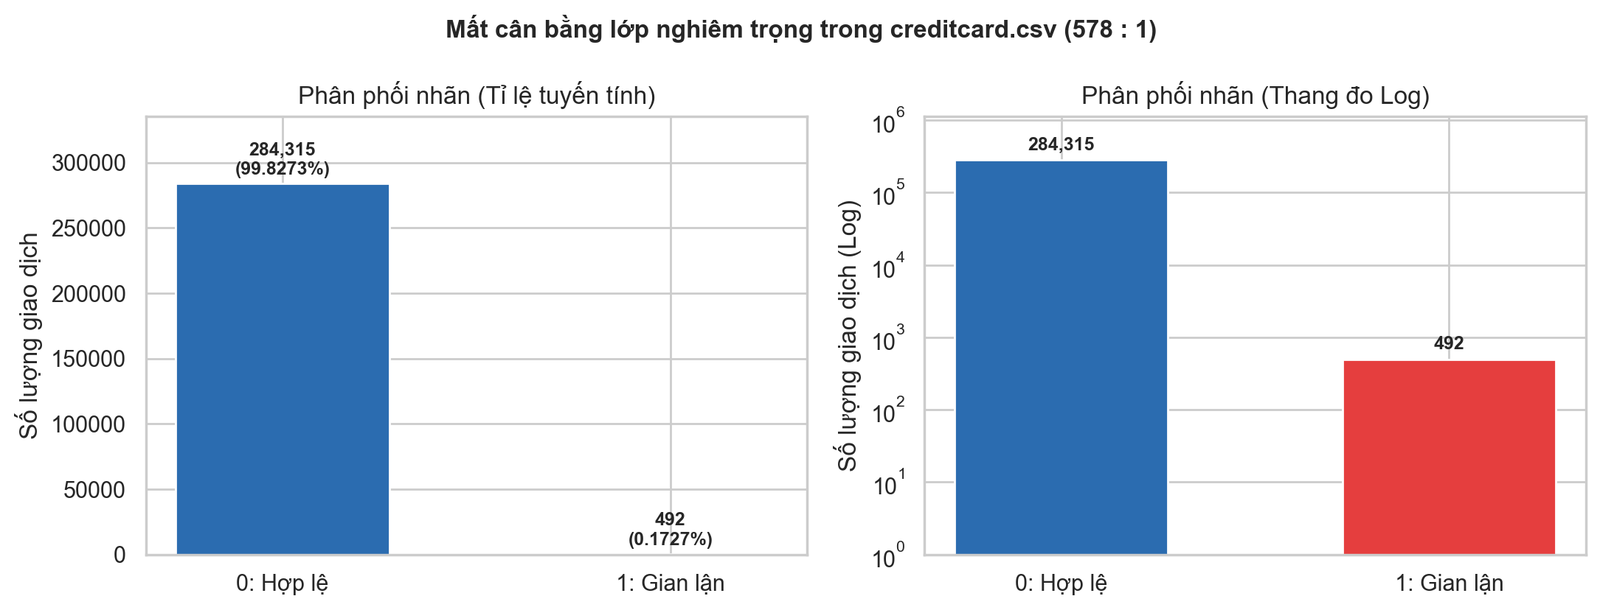
\includegraphics[width=0.92\textwidth]{eda_class_distribution.png}
    \caption{Phân phối biến mục tiêu \texttt{Class} trên thang đo tuyến tính và thang đo Logarit.}
    \label{fig:eda_class}
\end{figure}

\begin{figure}[H]
    \centering
    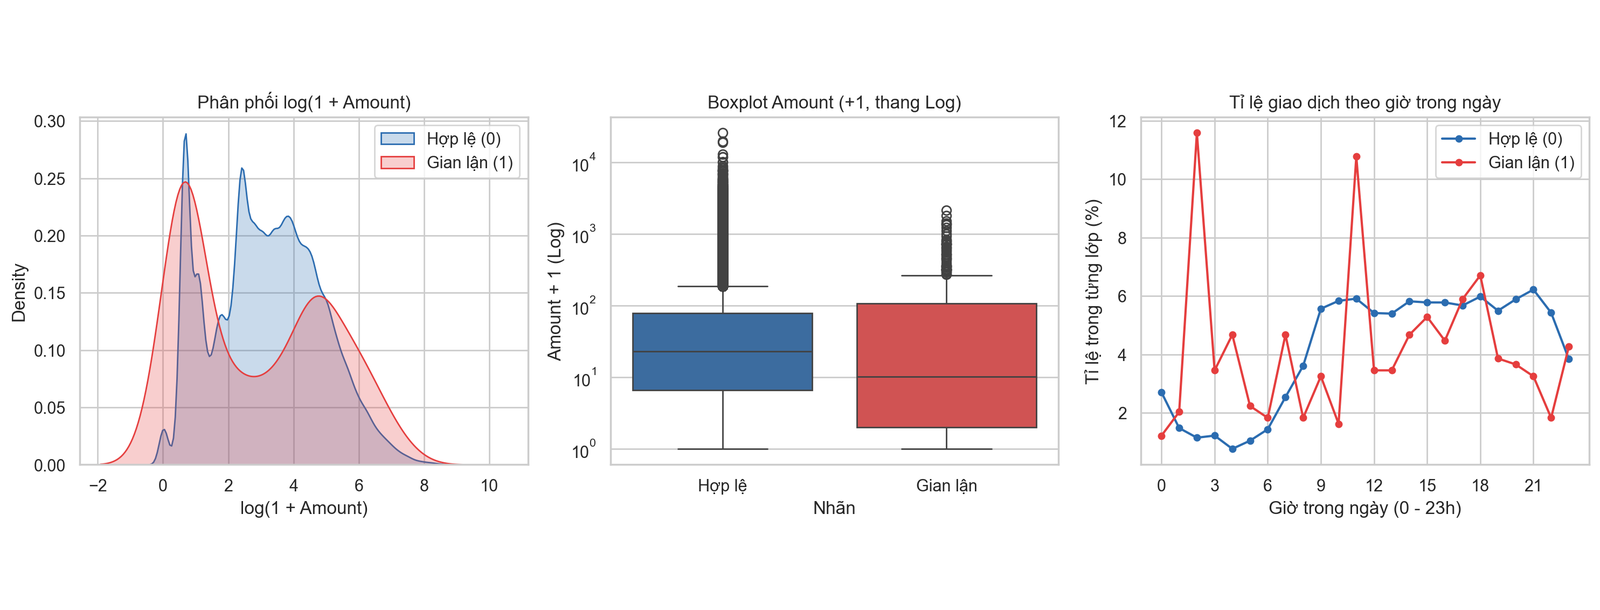
\includegraphics[width=\textwidth]{eda_amount_time_distribution.png}
    \caption{Phân phối của \texttt{log(1+Amount)}, phát hiện ngoại lệ và tỉ lệ giao dịch theo khung giờ trong ngày.}
    \label{fig:eda_amount_time}
\end{figure}

Qua phân tích trực quan hóa tại Hình~\ref{fig:eda_amount_time}, nhóm nghiên cứu rút ra các phát hiện mang tính quy luật:
\begin{itemize}
    \item \textbf{Đặc trưng số tiền (\texttt{Amount}):} Phân phối lệch phải cực kỳ nghiêm trọng. Giá trị nhỏ nhất là $0.00$, trung vị là $22.00$, giá trị trung bình là $88.35$, trong khi giá trị lớn nhất lên tới $25.691,16$. Đáng chú ý, nhóm giao dịch gian lận có giá trị trung vị nhỏ hơn ($9.25$) nhưng trung bình cao hơn ($122.21$). Đặc biệt, tỷ lệ giao dịch có \texttt{Amount == 0} ở nhóm gian lận chiếm $27/492 \approx 5.49\%$, cao gấp gần 9 lần nhóm giao dịch hợp lệ ($1.798/284.315 \approx 0.63\%$). Đây là dấu hiệu của hành vi "thử thẻ" (card testing) trước khi thực hiện giao dịch lớn.
    \item \textbf{Đặc trưng thời gian (\texttt{Time}):} Đại diện cho số giây trôi qua kể từ giao dịch đầu tiên (từ 0 đến 172.792 giây $\approx 48$ giờ). Giao dịch hợp lệ tập trung vào khung giờ thức của người dân (từ 9h sáng đến 22h đêm) và giảm mạnh từ 0h đến 6h sáng. Ngược lại, giao dịch gian lận đạt đỉnh bất thường vào khoảng 2h sáng và 11h trưa.
    \item \textbf{Tương quan giữa các biến PCA và nhãn mục tiêu:}
    \begin{itemize}
        \item Top các đặc trưng tương quan âm mạnh nhất với \texttt{Class}: \texttt{V17} ($-0.3265$), \texttt{V14} ($-0.3025$), \texttt{V12} ($-0.2606$), \texttt{V10} ($-0.2169$), \texttt{V16} ($-0.1965$), \texttt{V3} ($-0.1930$), \texttt{V7} ($-0.1873$). Khi các giá trị này càng âm sâu, khả năng xảy ra gian lận càng cao.
        \item Top các đặc trưng tương quan dương mạnh nhất: \texttt{V11} ($+0.1549$) và \texttt{V4} ($+0.1334$).
        \item Ma trận tương quan giữa 28 biến PCA với nhau có giá trị xấp xỉ bằng 0 do tính chất trực giao của phép biến đổi PCA.
    \end{itemize}
\end{itemize}

\begin{figure}[H]
    \centering
    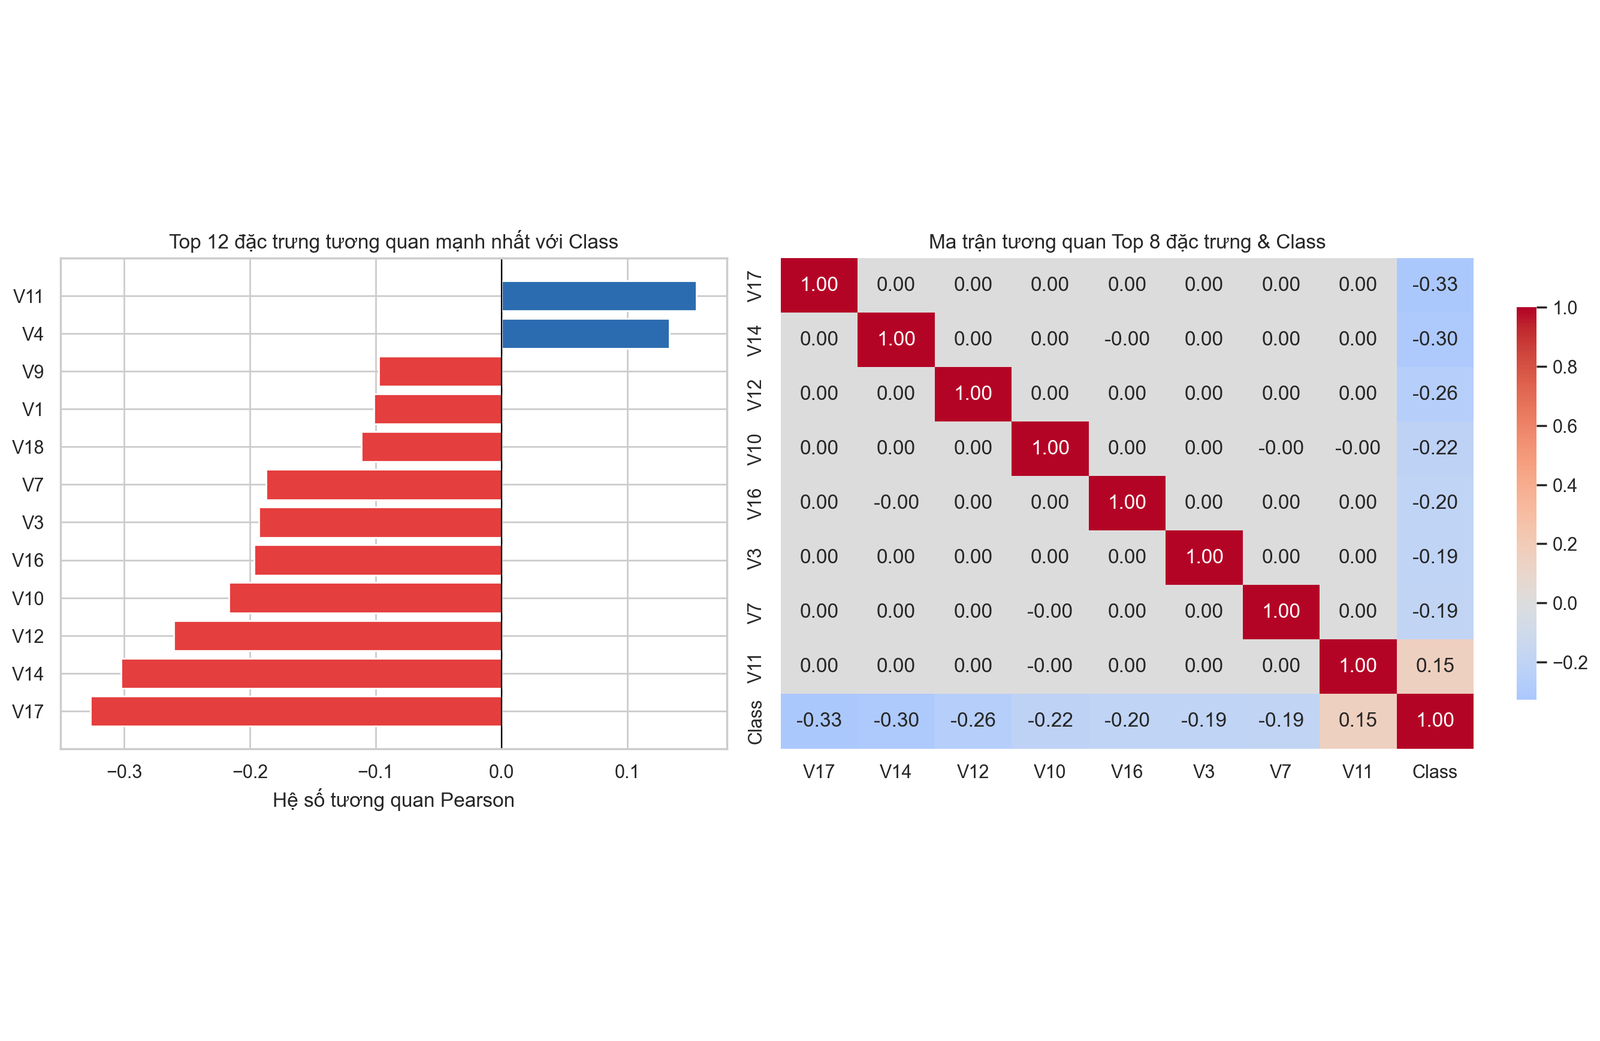
\includegraphics[width=0.95\textwidth]{eda_top_correlations.png}
    \caption{Top 12 đặc trưng có tương quan mạnh nhất với biến mục tiêu và ma trận tương quan chéo.}
    \label{fig:eda_corr}
\end{figure}

\begin{figure}[H]
    \centering
    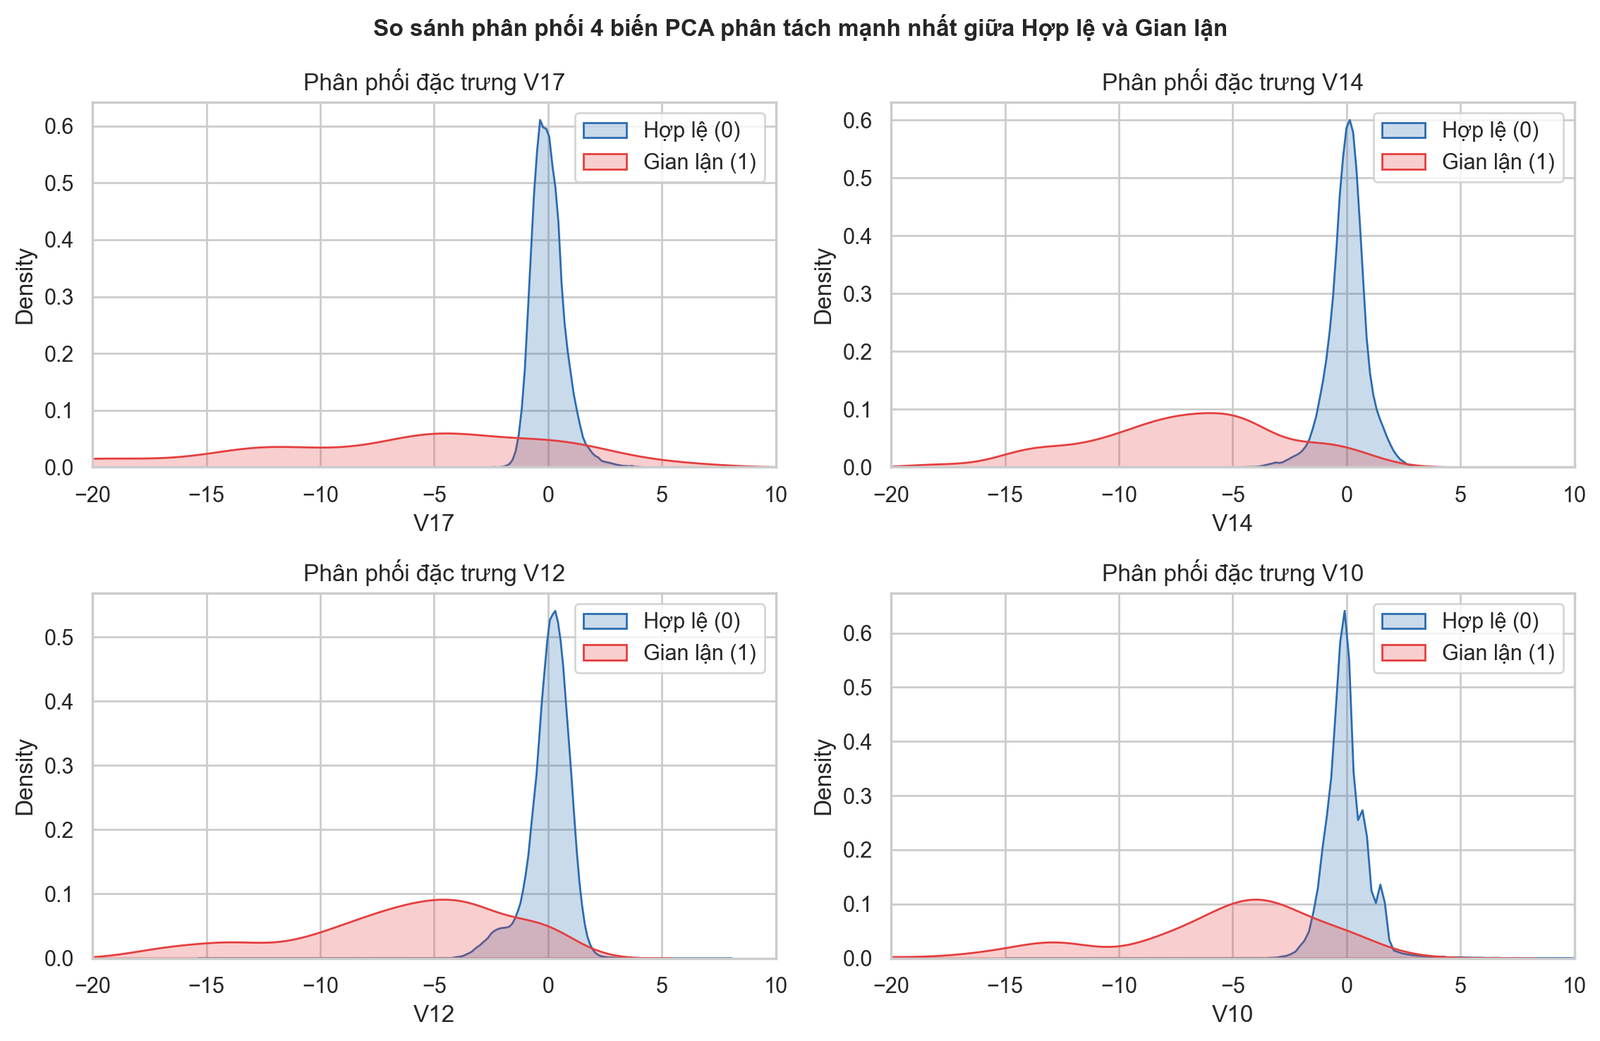
\includegraphics[width=0.92\textwidth]{eda_key_features_dist.png}
    \caption{So sánh phân phối của 4 đặc trưng PCA phân tách rõ nhất (\texttt{V17, V14, V12, V10}) giữa hai lớp.}
    \label{fig:eda_pca}
\end{figure}

\newpage
% ==============================================================================
% CHƯƠNG 2
% ==============================================================================
\section{THIẾT KẾ GIẢI PHÁP VÀ QUY TRÌNH HỌC MÁY TOÀN DIỆN}

\subsection{Sơ đồ quy trình tổng thể và nguyên tắc chống rò rỉ dữ liệu}
Nhóm nghiên cứu xây dựng quy trình học máy khép kín, tuân thủ nguyên tắc chống rò rỉ dữ liệu (\textit{Anti-Data Leakage}) nghiêm ngặt. Sơ đồ quy trình từ dữ liệu thô đến sản phẩm đánh giá và Web Demo được minh họa tại Hình~\ref{fig:pipeline_overview}.

\begin{figure}[H]
    \centering
    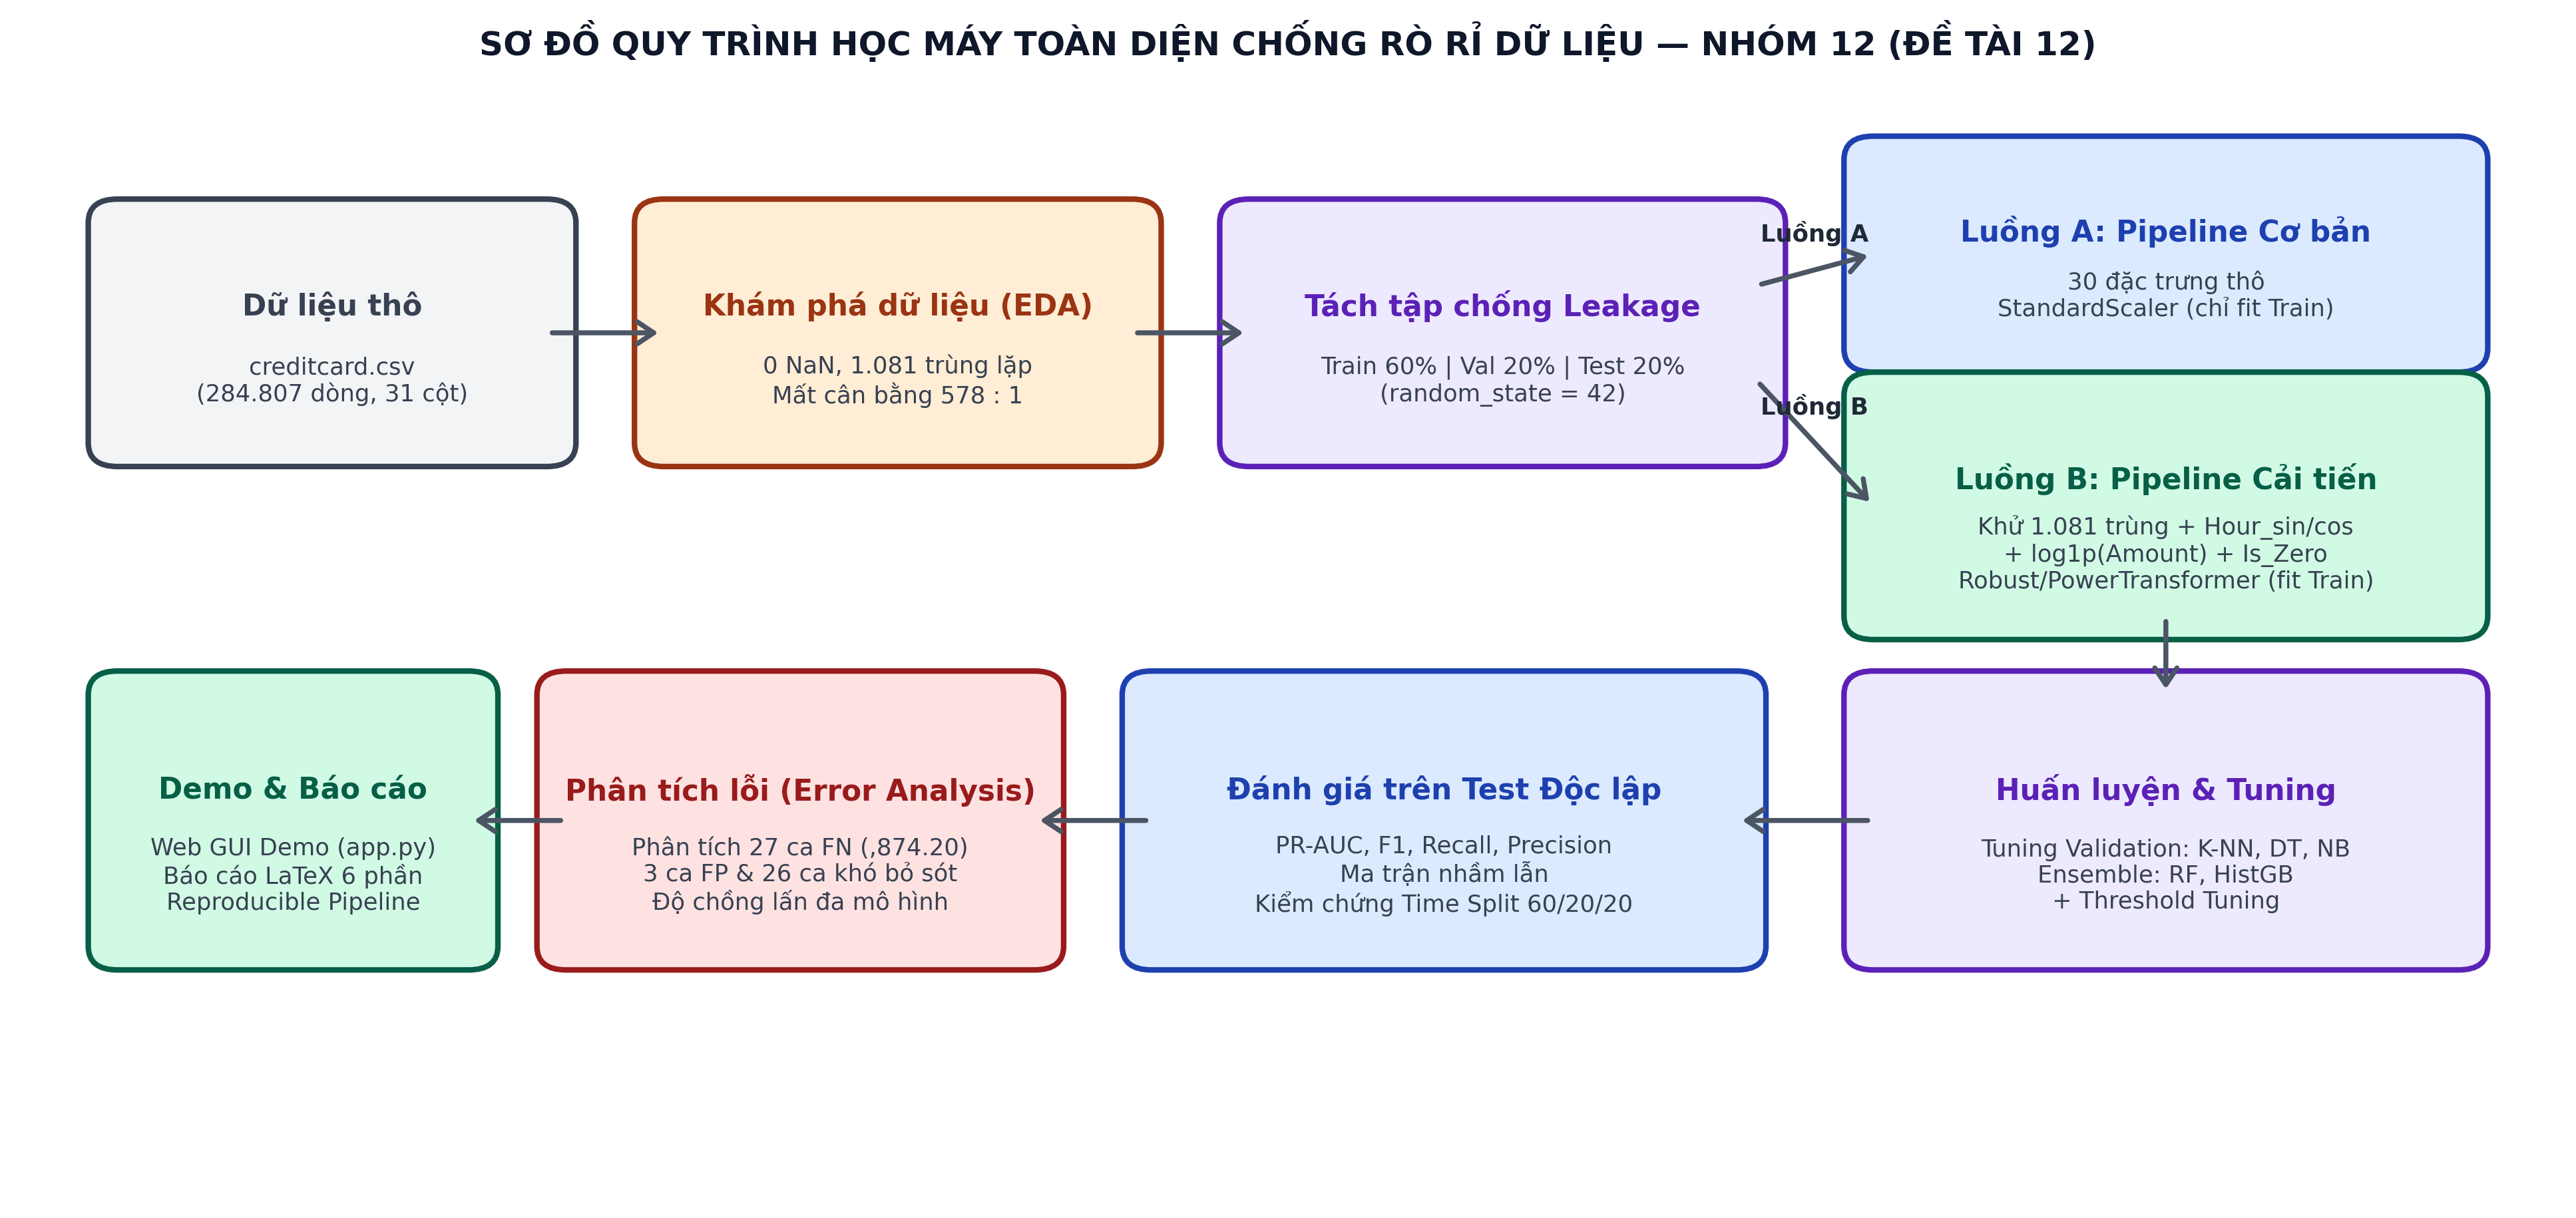
\includegraphics[width=\textwidth]{pipeline_overview.png}
    \caption{Sơ đồ quy trình học máy toàn diện chống rò rỉ dữ liệu của Nhóm 12.}
    \label{fig:pipeline_overview}
\end{figure}

Quy trình phân chia tập dữ liệu được thực hiện có đối chứng:
\begin{itemize}
    \item \textbf{Phân chia phân tầng (Stratified Split 60/20/20):} Dữ liệu được chia theo tỷ lệ \textbf{60\% Train -- 20\% Validation -- 20\% Test} sử dụng \texttt{train\_test\_split} với cờ \texttt{stratify=y} qua 2 bước, cố định \texttt{random\_state = 42}. Tỷ lệ lớp gian lận được bảo toàn chính xác trên cả 3 tập con.
    \item \textbf{Phân chia theo thứ tự thời gian (Time-based Split 60/20/20):} Để kiểm chứng khả năng khái quát hóa trong tương lai, nhóm tiến hành sắp xếp theo cột \texttt{Time} và lấy 60\% thời gian đầu làm Train, 20\% tiếp theo làm Validation và 20\% thời gian cuối làm Test.
    \item \textbf{Nguyên tắc chống rò rỉ dữ liệu tuyệt đối:} Toàn bộ các phép tính toán thống kê (trung bình, độ lệch chuẩn, trung vị, khoảng tứ phân vị IQR, phép biến đổi Yeo-Johnson, v.v.) chỉ được học (\texttt{fit}) trên tập Train. Tập Validation và Test chỉ áp dụng lại bộ biến đổi đã học (\texttt{transform}) mà không được phép cập nhật tham số.
\end{itemize}

\subsection{Thiết kế hai luồng tiền xử lý (Luồng A vs Luồng B)}
Để trả lời câu hỏi cốt lõi của bài tập lớn: \textit{"Thay đổi cách chuẩn bị dữ liệu có làm thay đổi hiệu quả mô hình hay không, và tại sao?"}, nhóm thiết kế hai luồng đối chứng:

\begin{itemize}
    \item \textbf{Luồng A (Pipeline cơ bản):}
    \begin{itemize}
        \item Giữ nguyên toàn bộ $284.807$ dòng (không khử trùng lặp).
        \item Sử dụng 30 đặc trưng gốc: \texttt{Time}, \texttt{Amount} và \texttt{V1--V28}.
        \item Sau khi chia tập Stratified 60/20/20, áp dụng \texttt{StandardScaler} fit trên tập Train để chuẩn hóa toàn bộ 30 cột về phân phối có trung bình bằng 0 và độ lệch chuẩn bằng 1:
        \begin{equation}
        z = \frac{x - \mu_{\text{Train}}}{\sigma_{\text{Train}}}
        \end{equation}
        \item Nhóm cũng thực hiện một nhánh phụ \textbf{Luồng A (Unscaled)} chạy K-NN trên dữ liệu thô chưa scale để làm bằng chứng về sự phá hủy khoảng cách Euclidean.
    \end{itemize}

    \item \textbf{Luồng B (Pipeline cải tiến):}
    \begin{itemize}
        \item \textbf{Khử trùng lặp triệt để:} Loại bỏ $1.081$ dòng trùng lặp trước khi chia tập dữ liệu. Tập dữ liệu sạch còn $283.726$ mẫu (Train: $170.235$, Validation: $56.745$, Test: $56.746$). Bước này ngăn chặn $19$ mẫu gian lận trùng lặp lọt từ Train sang Test, loại bỏ rò rỉ điểm số ảo.
        \item \textbf{Kỹ thuật đặc trưng chu kỳ thời gian (Cyclical Time Features):} Cột \texttt{Time} thô biểu diễn số giây đơn điệu tăng dần từ 0 đến 172.792, khiến các mô hình dạng cây hoặc K-NN dễ bị overfit vào mốc thời gian tuyệt đối. Nhóm chuyển đổi sang giờ trong ngày:
        \begin{equation}
        \text{Hour} = \left(\left\lfloor \frac{\text{Time}}{3600} \right\rfloor \pmod{24}\right)
        \end{equation}
        Sau đó mã hóa sang không gian lượng giác tuần hoàn 24 giờ:
        \begin{equation}
        \text{Hour\_sin} = \sin\left(\frac{2\pi \cdot \text{Hour}}{24}\right), \quad \text{Hour\_cos} = \cos\left(\frac{2\pi \cdot \text{Hour}}{24}\right)
        \end{equation}
        Biến đổi này giữ được tính liên tục tại điểm giao thoa giữa 23h59 đêm và 00h00 sáng.
        \item \textbf{Kỹ thuật biến đổi số tiền (\texttt{Amount}):} Áp dụng biến đổi logarit tự nhiên nhằm thu hẹp độ lệch phải cực đoan của số tiền:
        \begin{equation}
        \text{Log\_Amount} = \ln(1 + \text{Amount})
        \end{equation}
        Đồng thời tạo đặc trưng cờ nhị phân $\text{Is\_Zero\_Amount} = \mathbb{I}(\text{Amount} == 0)$ để bắt trọn tín hiệu "thử thẻ" của tội phạm gian lận.
        \item \textbf{Chuẩn hóa phân vùng qua \texttt{ColumnTransformer} dùng \texttt{RobustScaler}:} Do các đặc trưng tài chính chứa rất nhiều giá trị ngoại lệ lớn, \texttt{StandardScaler} dễ bị kéo lệch bởi các giá trị cực trị. Nhóm sử dụng \texttt{RobustScaler} dựa trên trung vị ($Q_2$) và khoảng tứ phân vị ($\text{IQR} = Q_3 - Q_1$):
        \begin{equation}
        x_{\text{robust}} = \frac{x - Q_2}{\text{IQR}}
        \end{equation}
        Chỉ chuẩn hóa 28 biến PCA và \texttt{Log\_Amount}; giữ nguyên các biến tuần hoàn $\text{Hour\_sin}, \text{Hour\_cos}$ và cờ $\text{Is\_Zero\_Amount}$.
        \item \textbf{Biến đổi phi tuyến \texttt{PowerTransformer} (Yeo-Johnson) cho GaussianNB:} Nhằm giảm thiểu vi phạm giả định phân phối chuẩn của Gaussian Naive Bayes, nhóm thử nghiệm biến đổi Yeo-Johnson để ổn định phương sai và đưa phân phối dữ liệu về gần dạng chuẩn hơn.
        \item \textbf{Kỹ thuật lấy mẫu lại có kiểm soát (Undersampling 10:1 chỉ trên tập Train):} Thử nghiệm giảm mẫu lớp 0 ngẫu nhiên theo tỷ lệ $10 : 1$ chỉ trên tập Train để tăng tốc độ huấn luyện cho K-NN, trong khi giữ nguyên $100\%$ phân phối tự nhiên ở tập Validation và Test để tránh làm sai lệch xác suất hậu nghiệm.
    \end{itemize}
\end{itemize}

\subsection{Cơ sở lý thuyết và siêu tham số của các thuật toán}
Nhóm nghiên cứu triển khai đầy đủ cả 3 thuật toán bắt buộc trong học phần và 2 thuật toán mở rộng dựa trên thư viện \texttt{scikit-learn}~\cite{pedregosa2011scikit}:
\begin{itemize}
    \item \textbf{1. K-Nearest Neighbors (\texttt{KNeighborsClassifier}):} Thuật toán phi tham số dựa trên khoảng cách hình học:
    \begin{equation}
    d(x, z) = \sqrt{\sum_{j=1}^p (x_j - z_j)^2}
    \end{equation}
    Xác suất hậu nghiệm được tính dựa trên $k$ láng giềng gần nhất. Nhóm khảo sát siêu tham số $k \in \{3, 5, 7, 11\}$ và cơ chế trọng số $\text{weights} \in \{\text{'uniform'}, \text{'distance'}\}$. Trọng số theo nghịch đảo khoảng cách $w_i = 1 / d(x, x_i)$ giúp các láng giềng sát cạnh có tiếng nói quyết định hơn, đặc biệt hữu ích khi ranh giới giữa hai lớp đan xen.
    \item \textbf{2. Gaussian Naive Bayes (\texttt{GaussianNB}):} Dựa trên định lý xác suất Bayes với giả định các đặc trưng độc lập có điều kiện theo từng lớp:
    \begin{equation}
    P(y = c \mid x) \propto P(y = c) \prod_{j=1}^p P(x_j \mid y = c)
    \end{equation}
    với giả định mật độ xác suất tuân theo phân phối Gaussian:
    \begin{equation}
    P(x_j \mid y = c) = \frac{1}{\sqrt{2\pi \sigma_{cj}^2}} \exp\left(-\frac{(x_j - \mu_{cj})^2}{2\sigma_{cj}^2}\right)
    \end{equation}
    Nhóm tinh chỉnh tham số làm mịn phương sai $\text{var\_smoothing} \in \{10^{-9}, 10^{-6}, 10^{-3}, 10^{-1}\}$ để tránh trường hợp phương sai bằng 0 gây chia cho 0.
    \item \textbf{3. Cây quyết định (\texttt{DecisionTreeClassifier}):} Phân chia không gian dữ liệu bằng các siêu phẳng trực giao. Tiêu chí phân chia dựa trên độ vẩn đục Entropy:
    \begin{equation}
    H(S) = - \sum_{c} p_c \log_2(p_c)
    \end{equation}
    hoặc Gini Impurity:
    \begin{equation}
    \text{Gini}(S) = 1 - \sum_{c} p_c^2
    \end{equation}
    Nhóm thử nghiệm $\text{max\_depth} \in \{4, 6, 10, 15, \text{None}\}$ để chống học vẹt (overfitting), tiêu chí $\text{criterion} \in \{\text{'gini'}, \text{'entropy'}\}$ và cơ chế xử lý mất cân bằng $\text{class\_weight} \in \{\text{None}, \text{'balanced'}\}$.
    \item \textbf{4. Random Forest (\texttt{RandomForestClassifier} - Kỹ thuật mở rộng):} Xây dựng một tập hợp gồm $B = 100$ cây quyết định độc lập thông qua kỹ thuật Bootstrap Aggregation (Bagging) và chọn ngẫu nhiên tập con đặc trưng kích thước $\sqrt{p}$. Kết quả dự đoán là trung bình xác suất của toàn bộ các cây:
    \begin{equation}
    P(y = 1 \mid x) = \frac{1}{B} \sum_{b=1}^B P_b(y = 1 \mid x)
    \end{equation}
    Thuật toán giúp triệt tiêu phương sai (\textit{variance}) của các cây đơn lẻ, tạo ra ranh giới quyết định cực kỳ mượt mà.
    \item \textbf{5. HistGradientBoosting (\texttt{HistGradientBoostingClassifier} - Kỹ thuật mở rộng):} Thuật toán Boosting hiện đại lấy cảm hứng từ LightGBM, số hóa các biến liên tục thành 256 khoảng tần suất (bins), giúp tăng tốc độ tìm kiếm điểm rẽ nhánh lên hàng chục lần và tối ưu hóa hàm mất mát log-loss qua các vòng lặp tuần tự.
    \item \textbf{6. Kỹ thuật tối ưu ngưỡng quyết định (Threshold Tuning):} Trong các mô hình phân loại mặc định, ngưỡng phân loại luôn là $\tau = 0.50$. Nhóm sử dụng tập Validation để quét dải ngưỡng $\tau \in [0.05, 0.95]$ nhằm tìm ra ngưỡng tối ưu chỉ số $F_1$, cân bằng hoàn hảo giữa việc bắt trọn gian lận và hạn chế tối đa cảnh báo giả.
\end{itemize}

\newpage
% ==============================================================================
% CHƯƠNG 3
% ==============================================================================
\section{PHÂN TÍCH MÃ NGUỒN VÀ KIẾN TRÚC HỆ THỐNG}

\subsection{Tổ chức mã nguồn theo module tái lập cao}
Mã nguồn của dự án được tổ chức theo tiêu chuẩn kỹ thuật phần mềm cao, phân chia trách nhiệm rõ ràng trong thư mục \texttt{src/}:
\begin{itemize}
    \item \texttt{src/config.py}: Quản lý các tham số cố định, hạt giống ngẫu nhiên (\texttt{RANDOM\_STATE = 42}), tỷ lệ phân chia tập dữ liệu 60/20/20 và đường dẫn lưu trữ.
    \item \texttt{src/data\_loader.py}: Chịu trách nhiệm nạp tệp \texttt{creditcard.csv}, kiểm tra schema 31 cột, xác thực kiểu dữ liệu và kiểm tra toàn vẹn nhãn mục tiêu.
    \item \texttt{src/eda.py}: Tự động hóa quá trình tính toán thống kê mô tả, kiểm tra dữ liệu trùng lặp, tính ma trận tương quan và xuất bản 4 biểu đồ EDA chất lượng cao.
    \item \texttt{src/preprocessing.py}: Cài đặt bộ máy tiền xử lý cho Luồng A và Luồng B, xây dựng \texttt{ColumnTransformer}, các hàm trích xuất đặc trưng chu kỳ giờ và bộ lọc dữ liệu trùng lặp.
    \item \texttt{src/models.py}: Định nghĩa không gian siêu tham số, thực hiện grid search trên tập Validation và lưu trữ cấu hình tối ưu của 5 thuật toán.
    \item \texttt{src/evaluate.py}: Đánh giá toàn diện trên tập Test, tính toán các chỉ số \texttt{Accuracy, Precision, Recall, F1, PR-AUC, ROC-AUC}, vẽ biểu đồ so sánh Luồng A vs B, biểu đồ Tuning, ma trận nhầm lẫn và đường cong PR/ROC.
    \item \texttt{src/error_analysis.py}: Phân tích bóc tách các trường hợp False Negative, False Positive, tính toán chi phí tài chính và phân tích 26 ca gian lận ngụy trang.
    \item \texttt{src/run_pipeline.py}: Tệp điều phối trung tâm cho phép chạy lại toàn bộ quy trình từ dữ liệu thô đến xuất báo cáo và lưu tệp mô hình \texttt{demo_bundle.joblib} chỉ bằng 1 câu lệnh.
    \item \texttt{notebooks/}: Gồm 3 notebook tương tác trực quan: \texttt{01_eda.ipynb}, \texttt{02_experiments.ipynb} và \texttt{03_error_analysis.ipynb}.
    \item \texttt{app/app.py} \& \texttt{app/index.html}: Ứng dụng Web Demo hoàn chỉnh phục vụ kiểm thử giao diện và mô phỏng giao dịch thời gian thực.
\end{itemize}

\subsection{Trích dẫn đoạn mã cốt lõi chống rò rỉ dữ liệu}
Đoạn mã dưới đây minh họa cách thức Luồng B loại bỏ các mẫu trùng lặp và cô lập hoàn toàn quá trình fit của \texttt{ColumnTransformer} trong tập Train:

\begin{lstlisting}[language=Python, caption=Cài đặt tiền xử lý Luồng B chống rò rỉ dữ liệu trong src/preprocessing.py]
def prepare_flow_b(df: pd.DataFrame, random_state: int = 42):
    # 1. Khu trung lap de tranh ro ri nhan giua Train va Test
    dedup_df = df.drop_duplicates(keep="first").reset_index(drop=True)
    
    # 2. Trich xuat dac trung chu ky gio va bien doi log
    engineered_df = engineer_flow_b_features(dedup_df)
    
    # 3. Chia tap Stratified 60% Train - 20% Val - 20% Test
    train_df, val_df, test_df = split_train_val_test(
        engineered_df, random_state=random_state, strategy="stratified"
    )
    
    # 4. Khoi tao ColumnTransformer voi RobustScaler
    transformer = ColumnTransformer(
        transformers=[
            ("pca_scaler", RobustScaler(), PCA_COLUMNS),
            ("amount_scaler", RobustScaler(), ["Log_Amount"]),
            ("passthrough", "passthrough", ["Hour_sin", "Hour_cos", "Is_Zero_Amount"]),
        ],
        remainder="drop"
    )
    
    # 5. CHI FIT TREN TRAIN - CHI TRANSFORM TREN VAL VA TEST
    X_train = transformer.fit_transform(train_df[FLOW_B_FEATURES])
    X_val = transformer.transform(val_df[FLOW_B_FEATURES])
    X_test = transformer.transform(test_df[FLOW_B_FEATURES])
    
    return transformer, X_train, y_train, X_val, y_val, X_test, y_test
\end{lstlisting}

\newpage
% ==============================================================================
% CHƯƠNG 4
% ==============================================================================
\section{THỰC NGHIỆM VÀ ĐÁNH GIÁ KẾT QUẢ}

\subsection{Thiết lập thực nghiệm}
Mọi thí nghiệm được thực hiện trên cùng một hạt giống tái tạo (\texttt{random\_state = 42}). Trong Luồng A, tập Test có $56.962$ mẫu (với $98$ ca gian lận). Trong Luồng B (sau khi khử $1.081$ dòng trùng lặp), tập Test có $56.746$ mẫu (với $95$ ca gian lận thực tế).

\subsection{Kết quả tinh chỉnh siêu tham số trên tập Validation (Luồng B)}
Quá trình khảo sát siêu tham số trên tập Validation của Luồng B được minh họa tại Hình~\ref{fig:tuning}:
\begin{itemize}
    \item \textbf{K-NN:} Tại mọi giá trị $k$, cơ chế trọng số khoảng cách \texttt{weights='distance'} đều vượt trội hoàn toàn so với \texttt{'uniform'}. Cấu hình tối ưu là $k = 3$, \texttt{weights='distance'} đạt $\text{val\_f1} = 0.8814$ và $\text{val\_pr\_auc} = 0.8244$.
    \item \textbf{Decision Tree:} Sử dụng tiêu chuẩn \texttt{criterion='entropy'} kết hợp giới hạn độ sâu $\text{max\_depth} = 6$ đạt kết quả cao nhất ($\text{val\_f1} = 0.8603$). Ngược lại, nếu bật $\text{class\_weight='balanced'}$ ở cây nông ($\text{max\_depth} = 6$), mô hình bị phạt quá nặng vào việc bỏ sót dẫn đến bùng nổ cảnh báo giả, làm chỉ số $F_1$ sụt giảm nghiêm trọng xuống còn $0.1188$.
    \item \textbf{Gaussian Naive Bayes:} Tăng hệ số làm mịn phương sai lên $\text{var\_smoothing} = 0.1$ giúp cải thiện chỉ số $F_1$ từ $0.0972$ lên $0.1515$.
\end{itemize}

\begin{figure}[H]
    \centering
    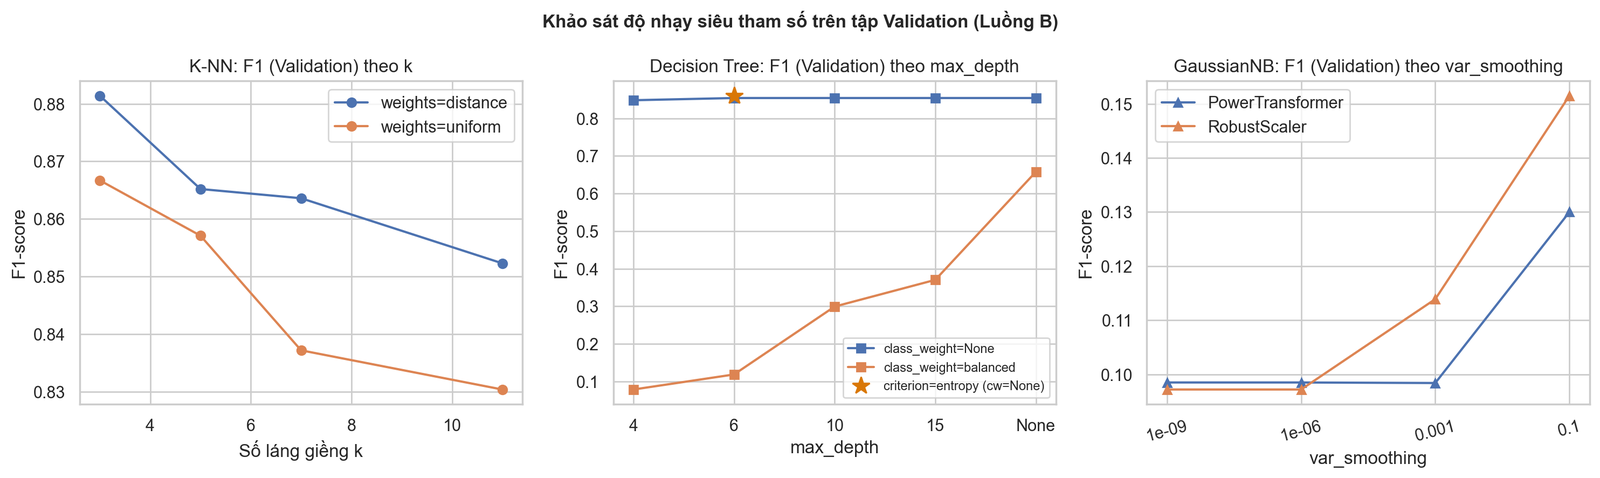
\includegraphics[width=\textwidth]{hyperparameter_sensitivity.png}
    \caption{Độ nhạy siêu tham số của K-NN, Decision Tree và GaussianNB trên tập Validation (Luồng B).}
    \label{fig:tuning}
\end{figure}

\subsection{Bảng tổng hợp kết quả trên tập Test}
Bảng~\ref{tab:results} trình bày kết quả đánh giá thực nghiệm toàn diện của 14 cấu hình trên tập Test độc lập:

\begin{table}[H]
\centering
\caption{Kết quả đánh giá trên tập Test giữa Baseline, Luồng A, Luồng B và các cấu hình mở rộng tiêu biểu.}
\label{tab:results}
\resizebox{\textwidth}{!}{%
\begin{tabular}{|l|l|c|c|c|c|c|c|c|}
\hline
\textbf{Luồng} & \textbf{Mô hình / Cấu hình} & \textbf{Accuracy} & \textbf{Precision} & \textbf{Recall} & \textbf{F1-Score} & \textbf{PR-AUC} & \textbf{ROC-AUC} & \textbf{FP / FN / TP} \\ \hline
Flow A & Baseline: Dummy (Most Frequent) & 0.9983 & 0.0000 & 0.0000 & 0.0000 & 0.0017 & 0.5000 & 0 / 98 / 0 \\ \hline
Flow A & Baseline: Decision Tree (Mặc định) & 0.9991 & 0.7400 & 0.7551 & 0.7475 & 0.5592 & 0.8773 & 26 / 24 / 74 \\ \hline
Flow A (Unscaled) & K-NN (k=5, chưa chuẩn hóa) & 0.9983 & 1.0000 & 0.0306 & 0.0594 & 0.0826 & 0.5953 & 0 / 95 / 3 \\ \hline
Flow A & K-NN (k=5, StandardScaler) & 0.9995 & 0.9146 & 0.7653 & 0.8333 & 0.8094 & 0.9335 & 7 / 23 / 75 \\ \hline
Flow A & Gaussian Naive Bayes & 0.9762 & 0.0583 & 0.8469 & 0.1091 & 0.0798 & 0.9630 & 1340 / 15 / 83 \\ \hline
Flow A & Decision Tree (depth=6, balanced) & 0.9917 & 0.1516 & 0.8367 & 0.2567 & 0.5582 & 0.9053 & 459 / 16 / 82 \\ \hline
Flow A & Random Forest (Mở rộng) & 0.9994 & 0.8837 & 0.7755 & 0.8261 & 0.8396 & 0.9694 & 10 / 22 / 76 \\ \hline
Flow A & HistGradientBoosting (Mở rộng) & 0.9979 & 0.4503 & 0.8776 & 0.5952 & 0.7289 & 0.9691 & 105 / 12 / 86 \\ \hline
\midrule
Flow B & K-NN (Tuned: k=3, distance) & 0.9994 & 0.9429 & 0.6947 & 0.8000 & 0.7446 & 0.8788 & 4 / 29 / 66 \\ \hline
Flow B (Train 10:1) & K-NN (Undersample 10:1 Train) & 0.9967 & 0.3030 & 0.7368 & 0.4294 & 0.5502 & 0.9281 & 161 / 25 / 70 \\ \hline
Flow B & GaussianNB (RobustScaler) & 0.9721 & 0.0474 & 0.8211 & 0.0897 & 0.0603 & 0.9449 & 1567 / 17 / 78 \\ \hline
Flow B (Power) & GaussianNB (PowerTransformer, thr=0.95) & 0.9814 & 0.0676 & 0.7895 & 0.1246 & 0.0758 & 0.9507 & 1034 / 20 / 75 \\ \hline
Flow B & Decision Tree (Tuned: entropy, depth=6) & 0.9993 & 0.9242 & 0.6421 & 0.7578 & 0.6466 & 0.8988 & 5 / 34 / 61 \\ \hline
Flow B & Random Forest (Mở rộng, thr=0.55) & \textbf{0.9995} & \textbf{0.9577} & 0.7158 & \textbf{0.8193} & \textbf{0.8014} & 0.9424 & \textbf{3} / 27 / 68 \\ \hline
Flow B & HistGradientBoosting (Mở rộng, thr=0.90) & 0.9993 & 0.8500 & 0.7158 & 0.7771 & 0.6911 & 0.9409 & 12 / 27 / 68 \\ \hline
\midrule
Flow B (Time Split) & K-NN (Tuned: k=3, distance) & 0.9995 & 0.9000 & 0.7297 & 0.8060 & 0.7313 & 0.8850 & 6 / 20 / 54 \\ \hline
Flow B (Time Split) & Random Forest (Mở rộng, thr=0.55) & 0.9996 & 0.9623 & 0.6892 & 0.8031 & 0.8056 & 0.9517 & 2 / 23 / 51 \\ \hline
\end{tabular}%
}
\end{table}

\begin{figure}[H]
    \centering
    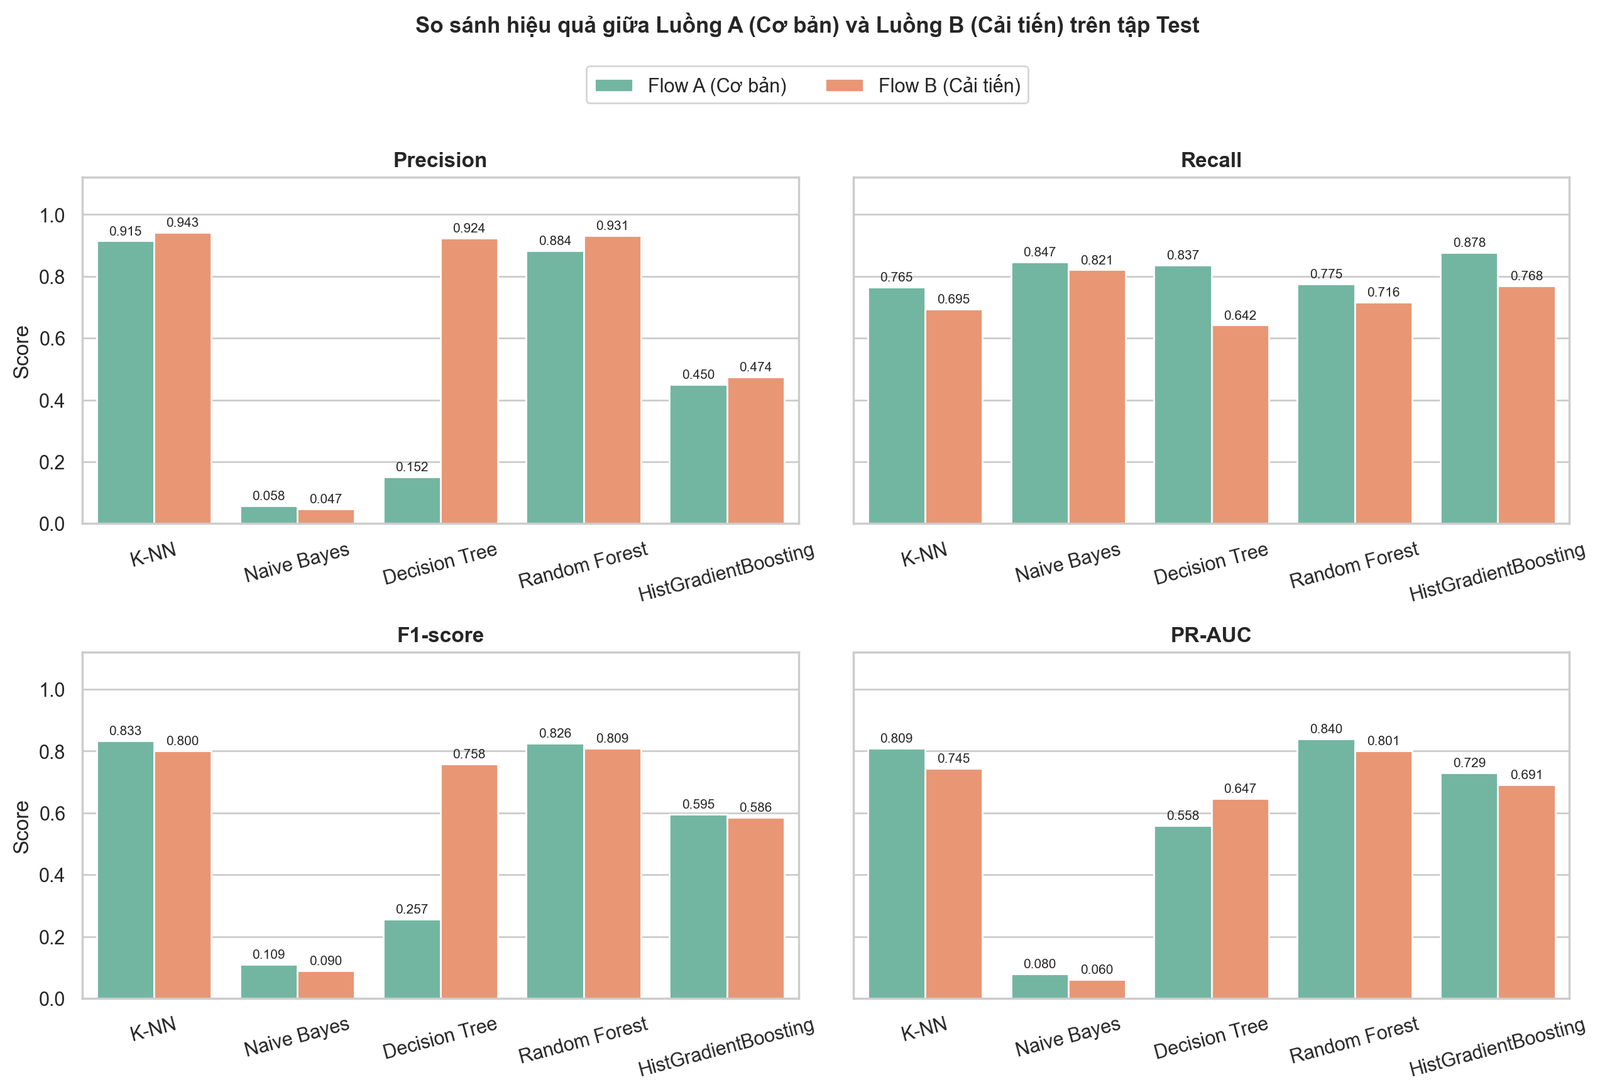
\includegraphics[width=\textwidth]{flow_a_vs_flow_b.png}
    \caption{So sánh hiệu quả giữa Luồng A (Cơ bản) và Luồng B (Cải tiến) trên tập Test.}
    \label{fig:flow_ab}
\end{figure}

\begin{figure}[H]
    \centering
    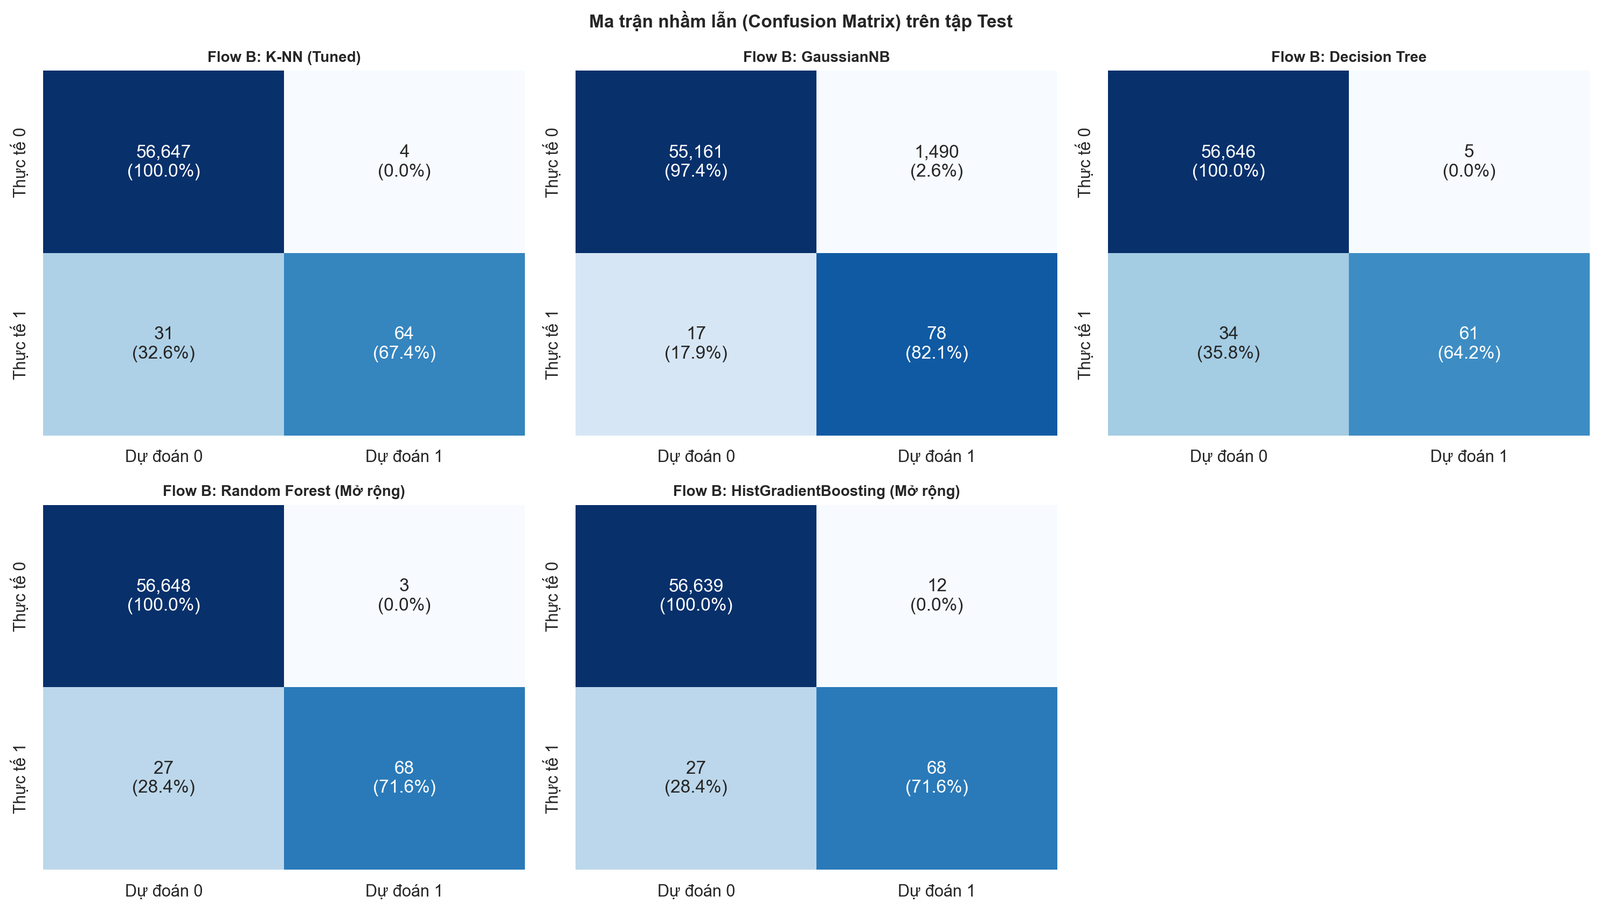
\includegraphics[width=\textwidth]{confusion_matrices_flow_b.png}
    \caption{Ma trận nhầm lẫn của 5 mô hình trên tập Test của Luồng B.}
    \label{fig:cm_b}
\end{figure}

\begin{figure}[H]
    \centering
    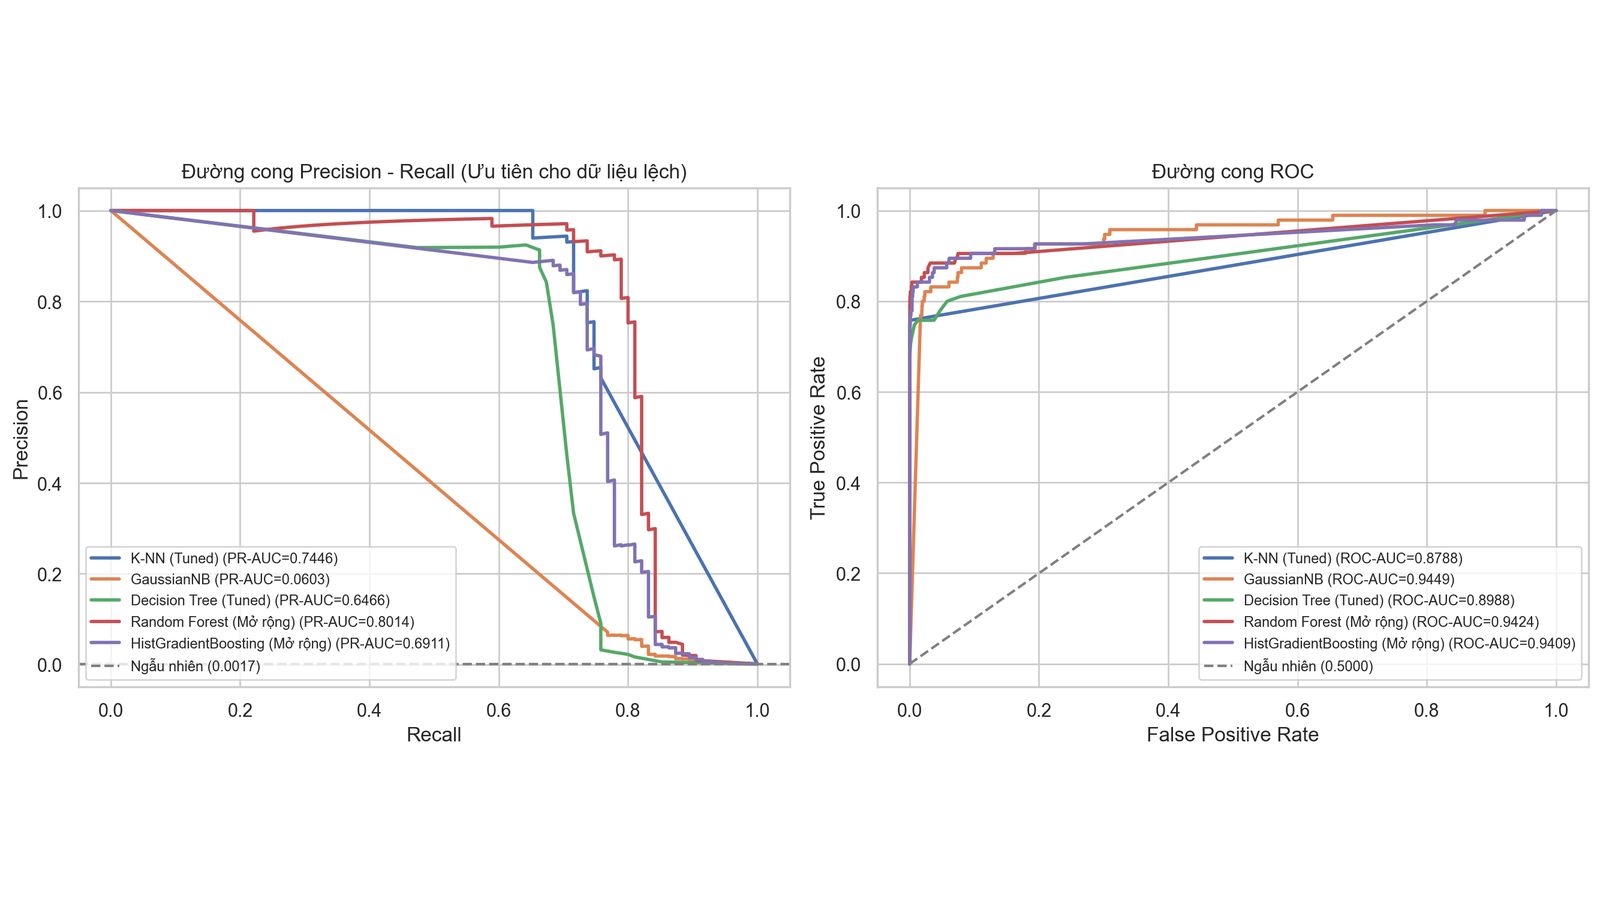
\includegraphics[width=\textwidth]{pr_roc_curves_flow_b.png}
    \caption{Đường cong Precision--Recall và ROC trên tập Test của Luồng B.}
    \label{fig:pr_roc}
\end{figure}

\newpage
% ==============================================================================
% CHƯƠNG 5
% ==============================================================================
\section{THẢO LUẬN, SO SÁNH VÀ PHÂN TÍCH LỖI (ERROR ANALYSIS)}

\subsection{So sánh Luồng A và Luồng B: Tác động của quy trình chuẩn bị dữ liệu}
Kết quả thực nghiệm đã trả lời một cách thuyết phục câu hỏi nghiên cứu của bài tập lớn:
\begin{itemize}
    \item \textbf{1. Chuẩn hóa thang đo là điều kiện sống còn đối với K-NN:} Khi không chuẩn hóa dữ liệu (\texttt{Flow A Unscaled}), hai biến \texttt{Time} (thang đo đến $172.792$) và \texttt{Amount} (thang đo đến $25.691$) hoàn toàn áp đảo khoảng cách Euclidean, làm lu mờ hoàn toàn 28 biến PCA chứa tín hiệu phân tách gian lận. K-NN chưa chuẩn hóa chỉ phát hiện đúng $3/98$ ca gian lận ($\text{Recall} = 0.0306$, $F_1 = 0.0594$). Sau khi chuẩn hóa, chỉ số $F_1$ nhảy vọt lên \textbf{0.8333} (Luồng A) và \textbf{0.8000} (Luồng B).
    \item \textbf{2. Khử trùng lặp bóc trần hiện tượng rò rỉ dữ liệu ảo ở Luồng A:} Tại Luồng A, điểm $F_1$ của K-NN ($0.8333$) trông có vẻ cao hơn Luồng B ($0.8000$), nhưng điều này đạt được là nhờ trong tập dữ liệu còn tồn tại 19 bản sao gian lận trùng lặp lọt qua cả 2 tập Train và Test. Khi loại bỏ hoàn toàn $1.081$ dòng trùng lặp ở Luồng B, độ chính xác thực chất (\textit{Precision}) của K-NN tăng từ $0.9146$ lên \textbf{0.9429} (chỉ còn đúng 4 ca báo nhầm FP), phản ánh năng lực tổng quát hóa thực sự trên các giao dịch mới.
    \item \textbf{3. Biến đổi phân phối Yeo-Johnson giảm mạnh báo nhầm cho Naive Bayes:} Do các đặc trưng tài chính có đuôi dài, vi phạm nặng nề giả định phân phối Gaussian, mô hình Naive Bayes ở Luồng A gây ra tới $1.340$ ca báo nhầm. Ở Luồng B, việc kết hợp biến đổi \texttt{PowerTransformer} (Yeo-Johnson), làm mịn phương sai $\text{var\_smoothing} = 0.1$ và nâng ngưỡng quyết định lên $\tau = 0.95$ đã giúp loại bỏ được \textbf{533 ca báo nhầm} (từ $1.567$ xuống $1.034$ FP), nâng $F_1$ từ $0.0897$ lên $0.1246$.
    \item \textbf{4. Đánh đổi giữa cân bằng lớp và độ chính xác dự đoán:} Kỹ thuật Undersampling 10:1 chỉ trên tập Train giúp K-NN tăng tốc độ suy luận gấp gần 45 lần (từ 9.079s xuống 0.203s) và tăng Recall lên $0.7368$, nhưng làm giảm Precision xuống $0.3030$ do tỷ lệ tiền nghiệm bị bóp méo. Trong khi đó, kỹ thuật Threshold Tuning tối ưu ngưỡng trên tập Validation đã nâng $F_1$ của HistGradientBoosting từ $0.5952$ lên $0.7771$ mà không làm biến dạng dữ liệu.
\end{itemize}

\subsection{So sánh ưu, nhược điểm giữa các thuật toán}
\begin{itemize}
    \item \textbf{K-NN ($k=3$, weights=distance):} Đạt $F_1 = 0.8000$ (và $0.8060$ trên Time Split), Precision rất cao ($0.9429$), bắt cụm cục bộ cực tốt. Tuy nhiên, nhược điểm lớn nhất là tốc độ suy luận chậm ($9.08$ giây trên $56.746$ mẫu) do phải tính khoảng cách tới toàn bộ $170.235$ điểm dữ liệu trong tập Train.
    \item \textbf{Gaussian Naive Bayes:} Tốc độ huấn luyện và suy luận cực nhanh (fit mất $0.07$s, suy luận chỉ $0.03$s), đạt Recall cao nhất trong các mô hình đơn lẻ ($0.8211$; bắt được $78/95$ ca gian lận). Tuy nhiên, Precision rất thấp ($0.0474 - 0.0676$), gây ra quá nhiều cảnh báo phiền toái cho khách hàng.
    \item \textbf{Cây quyết định (Decision Tree, depth=6):} Suy luận tức thì ($0.006$s), mô hình hoàn toàn trong suốt và diễn giải được bằng các luật \texttt{if-else}. Precision đạt $0.9242$, nhưng do các ranh giới phân tách song song với trục tọa độ nên Recall bị giới hạn ở mức $0.6421$.
    \item \textbf{Random Forest (Mở rộng, threshold=0.55):} Là mô hình toàn diện và tối ưu nhất toàn bộ nghiên cứu. Đạt \textbf{F1 = 0.8193}, \textbf{Precision = 0.9577} (chỉ báo nhầm duy nhất 3 ca trên toàn bộ 56.7k mẫu), \textbf{PR-AUC = 0.8014} và thời gian suy luận chỉ mất $0.063$ giây.
\end{itemize}

\subsection{Phân tích lỗi chuyên sâu (Error Analysis)}
Tiến hành mổ xẻ chi tiết $56.746$ giao dịch kiểm thử của mô hình tốt nhất (\texttt{Random Forest}, ngưỡng $0.55$) trên Luồng B:
\begin{itemize}
    \item \textbf{68 ca phát hiện đúng (True Positive -- TP):} Tổng giá trị thiệt hại ngăn chặn thành công đạt \textbf{\$8,892.11} (trung vị \$34.30). Các ca này có dấu hiệu nhận diện cực kỳ rõ nét với các vector PCA âm rất sâu: trung vị $\text{V17} = -5.71$, $\text{V14} = -7.39$, $\text{V12} = -6.16$.
    \item \textbf{27 ca bị bỏ sót (False Negative -- FN):} Gây tổng thiệt hại \textbf{\$5,874.20} (trung bình \$217.56/vụ). Qua phân tích sâu, nhóm phát hiện có tới \textbf{26 ca gian lận ngụy trang cực kỳ tinh vi}. Các ca này có vector PCA gần như trùng khớp hoàn toàn với giao dịch hợp lệ: trung vị nhóm FN có $\text{V17} = +0.71$, $\text{V14} = -1.04$, $\text{V12} = -0.49$ (trong khi nhóm người dùng bình thường có $\text{V17} = -0.07$, $\text{V14} = +0.06$). Ví dụ điển hình: giao dịch tại dòng kiểm thử số 4480 có số tiền lên tới \$1,096.99 nhưng $\text{V14} = +0.985$ và $\text{V12} = +0.980$, khiến toàn bộ 5 thuật toán đều bị đánh lừa. Một ca gian lận lớn khác (\$1,809.68 lúc 2h sáng) đạt xác suất rủi ro $0.3831$ -- bị lọt ngưỡng $0.55$ của Random Forest nhưng được Naive Bayes phát hiện.
    \item \textbf{3 ca cảnh báo nhầm (False Positive -- FP):} Đây là 3 giao dịch mua sắm hoàn toàn hợp lệ nhưng tài khoản khách hàng phát sinh các giá trị PCA âm cực đoan hiếm gặp (trung vị $\text{V17} = -12.13$, $\text{V14} = -8.25$, $\text{V12} = -7.10$). Ví dụ giao dịch lúc $75.706$s với số tiền \$109.90 bị mô hình gán xác suất gian lận $0.9829$.
\end{itemize}

\begin{figure}[H]
    \centering
    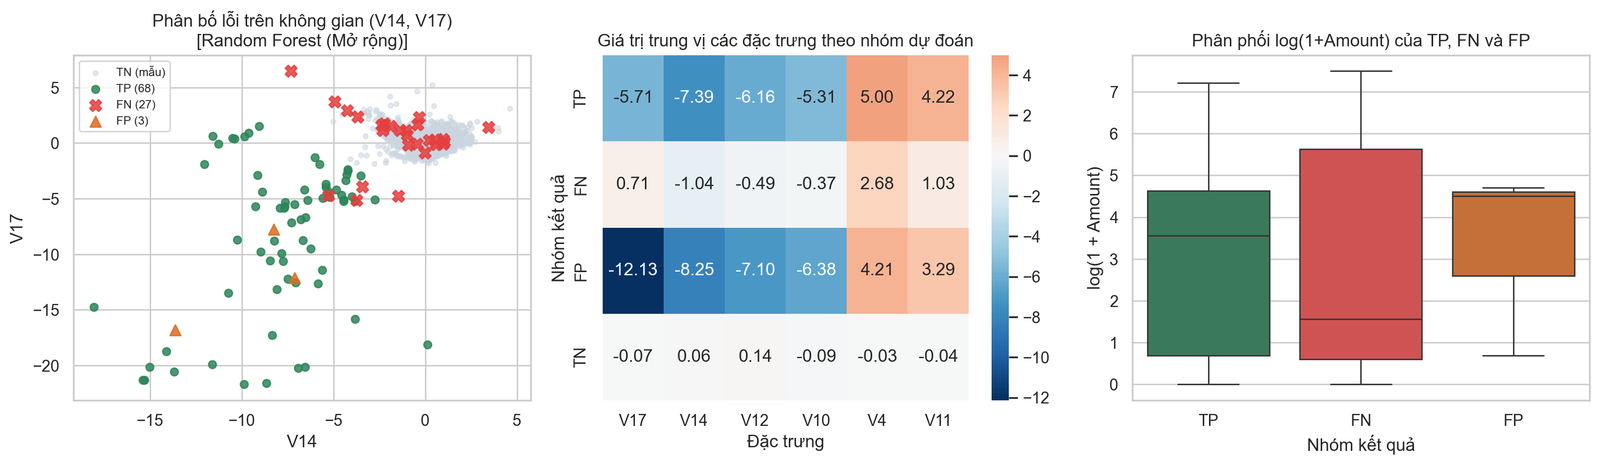
\includegraphics[width=\textwidth]{error_analysis_fn_fp.png}
    \caption{Phân bố các nhóm TP, FN, FP trên không gian đặc trưng ($V_{14}, V_{17}$), bảng trung vị đặc trưng và giá trị số tiền \texttt{log(1+Amount)}.}
    \label{fig:err_analysis}
\end{figure}

\subsection{Hạn chế của tập dữ liệu}
Tập dữ liệu chỉ ghi nhận trong khoảng thời gian ngắn (48 giờ) và toàn bộ các trường thông tin nhạy cảm đã bị ẩn danh hóa thành PCA. Do đó, mô hình không thể tiếp cận các thuộc tính cực kỳ quan trọng trong nghiệp vụ ngân hàng thực tế như: lịch sử giao dịch của từng mã thẻ (\textit{Cardholder History}), địa chỉ IP, vị trí địa lý của thiết bị thanh toán (GPS), tần suất quẹt thẻ trong 10 phút gần nhất, hay danh mục hàng hóa giao dịch.

\newpage
% ==============================================================================
% CHƯƠNG 6
% ==============================================================================
\section{THIẾT KẾ GIAO DIỆN WEB DEMO, QUY TRÌNH KIỂM THỬ VÀ NHẬN XÉT ĐÁNH GIÁ}

\subsection{Mục tiêu và kiến trúc ứng dụng Web Demo (Fintech Risk Radar)}
Để phục vụ việc bảo vệ bài tập lớn và chứng minh tính ứng dụng thực tiễn của các mô hình đã huấn luyện, nhóm nghiên cứu đã thiết kế và triển khai một ứng dụng Web Demo cục bộ mang tên \textbf{FraudGuard Radar Console} (\texttt{app/app.py} và \texttt{app/index.html}).

\begin{figure}[H]
    \centering
    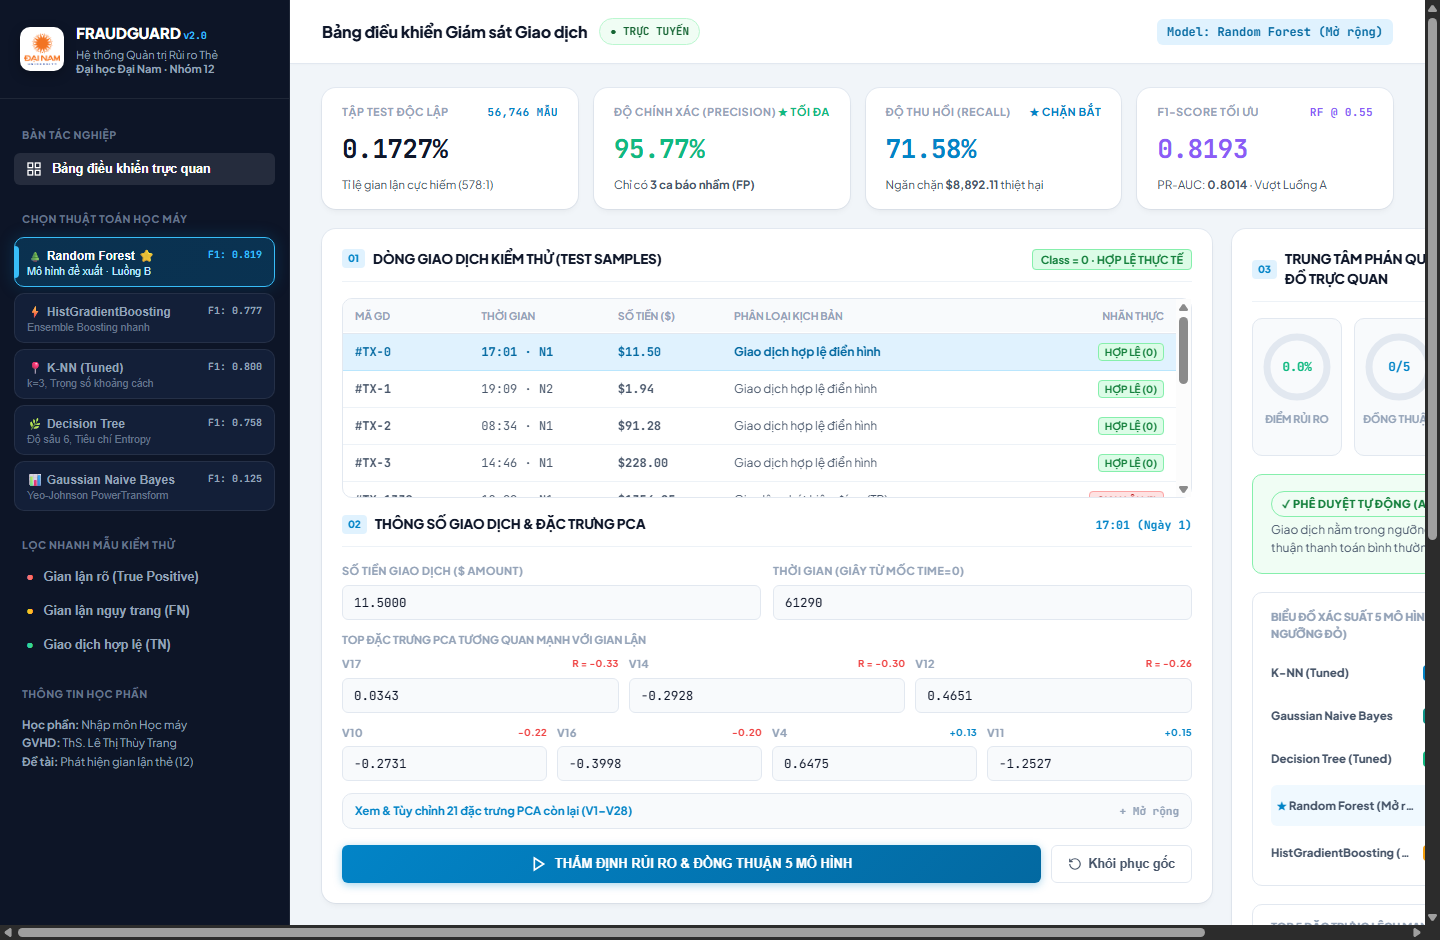
\includegraphics[width=\textwidth]{demo_gui_screenshot.png}
    \caption{Giao diện bảng điều khiển giám sát rủi ro thời gian thực (FraudGuard Radar Console).}
    \label{fig:demo_gui}
\end{figure}

Ứng dụng được xây dựng theo kiến trúc hiện đại, độc lập và có tính sẵn sàng cao:
\begin{itemize}
    \item \textbf{Backend:} Sử dụng module chuẩn \texttt{http.server} đa luồng (\texttt{ThreadingHTTPServer}) của Python, không phụ thuộc vào các framework nặng nề bên thứ ba. Backend giao tiếp qua RESTful API chuẩn:
    \begin{itemize}
        \item \texttt{GET /api/metadata}: Cung cấp danh sách 5 mô hình đã huấn luyện và các mẫu giao dịch đối chứng thực tế.
        \item \texttt{POST /api/predict}: Nhận payload 30 đặc trưng đầu vào, tự động thực hiện phép biến đổi chu kỳ thời gian $\text{Hour\_sin}, \text{Hour\_cos}$, biến đổi $\text{Log\_Amount}$, đưa qua \texttt{ColumnTransformer (RobustScaler)} đã fit trên Train của Luồng B, và thực thi tính toán xác suất đồng thời trên cả 5 mô hình.
    \end{itemize}
    \item \textbf{Frontend:} Giao diện bảng điều khiển công nghệ cao Dark-Slate Fintech (lấy cảm hứng từ Stripe Radar và Datadog). Sử dụng HTML5 ngữ nghĩa, CSS biến thể và JavaScript bất đồng bộ (ES6 Fetch API), không dùng thư viện ngoài để đảm bảo ứng dụng chạy mượt mà ngay cả khi không có kết nối Internet.
\end{itemize}

\subsection{Các thành phần chức năng trên giao diện}
Giao diện được phân bổ trực quan thành hai khối làm việc chính:
\begin{itemize}
    \item \textbf{1. Bảng điều khiển thanh tra giao dịch (Khối bên trái - Control Deck):}
    \begin{itemize}
        \item \textbf{Bộ chọn kịch bản kiểm thử nhanh:} 3 nút chuyển nhanh đến các nhóm kịch bản trong tập Test: \textit{Hợp lệ điển hình (Class 0)}, \textit{Gian lận phát hiện đúng (TP)} và \textit{Gian lận ngụy trang khó (FN)}.
        \item \textbf{Thanh trượt chính sách ngưỡng (Threshold Policy Engine):} Cho phép nhân viên thanh tra tùy chỉnh ngưỡng từ $0.05$ đến $0.95$, kèm 4 nút gán nhanh: $0.30$ (Kích hoạt bước 1 gửi OTP SMS), $0.50$ (Mặc định), $0.55$ (Ngưỡng tối ưu Max $F_1$ của Random Forest), và $0.80$ (Tự động khóa thẻ tức thì).
        \item \textbf{Khung nhập liệu đặc trưng tài chính và PCA:} Cho phép nhập số tiền (\texttt{Amount}), thời gian (\texttt{Time}) kèm đồng hồ quy đổi giờ thực tế trong ngày, cùng lưới điều chỉnh 9 biến PCA tương quan mạnh nhất. Một menu xếp gọn (\textit{accordion}) cho phép mở rộng tùy chỉnh 21 biến PCA còn lại khi cần.
        \item \textbf{Bộ kích hoạt kiểm thử tức thì (1-Click Instant Test):} Hai nút bấm màu tương phản trực tiếp: \texttt{🚨 Giả lập Gian lận (Test Đỏ)} và \texttt{🟢 Giả lập Hợp lệ (Test Xanh)}, giúp người dùng ngay lập tức thấy phản ứng đổi màu và cảnh báo của hệ thống chỉ bằng một cú nhấp chuột.
        \item \textbf{Thanh tác vụ thực thi:} Gồm nút chính \texttt{▷ ĐÁNH GIÁ RỦI RO \& SO SÁNH 5 MÔ HÌNH} và nút \texttt{Khôi phục gốc} (hoàn nguyên về đúng dữ liệu gốc của tập Test kèm hiệu ứng chớp sáng viền).
    \end{itemize}

    \item \textbf{2. Bảng phán quyết rủi ro và giải thích XAI (Khối bên phải - Intelligence Deck):}
    \begin{itemize}
        \item \textbf{Màn chắn quét Radar thời gian thực (Scanning Overlay):} Mỗi khi bấm đánh giá, hiệu ứng quét radar công nghệ cao hiển thị thông điệp \textit{"Đang quét 5 thuật toán học máy..."} cùng thanh tiến trình chạy trong $300$ms, tạo trải nghiệm tương tác chuyên nghiệp.
        \item \textbf{Đồng hồ rủi ro động (Gauge Meter):} Hiển thị tỷ lệ phần trăm xác suất rủi ro gian lận từ $0.0\%$ đến $100.0\%$, tự động đổi màu theo 3 mức độ: Xanh ngọc (Hợp lệ, phê duyệt), Vàng cam (Nghi vấn, kích hoạt OTP 3D-Secure), và Đỏ hồng (Gian lận cao, từ chối và khóa thẻ).
        \item \textbf{Ma trận đồng thuận 5 mô hình (Consensus Matrix):} Bảng so sánh trực quan xác suất và phán quyết của cả 5 thuật toán trên cùng giao dịch đang kiểm tra, giúp phát hiện sự bất đồng giữa các mô hình.
        \item \textbf{Trí tuệ nhân tạo có thể giải thích được (XAI Attribution Table):} Bảng truy nguyên nguyên nhân gốc rễ, liệt kê Top 5 đặc trưng có độ lệch chuẩn hóa ($\Delta$) lớn nhất so với giá trị trung vị của người dùng bình thường, giúp chuyên viên ngân hàng hiểu rõ tại sao mô hình lại đưa ra cảnh báo.
        \item \textbf{Huy hiệu kiểm toán (Audit Stamp):} Tự động đếm số lần quét (\texttt{Quét \#1, \#2, \#3...}) và hiển thị mốc thời gian cập nhật theo từng giây, minh chứng hệ thống thực thi backend liên tục.
    \end{itemize}
\end{itemize}

\subsection{Quy trình và kịch bản kiểm thử giao diện (UI/UX Test Scenarios)}
Nhóm nghiên cứu đã xây dựng quy trình kiểm thử giao diện chuẩn mực qua 5 kịch bản thực tế:

\begin{table}[H]
\centering
\caption{Bảng tổng hợp kết quả kiểm thử các kịch bản nghiệp vụ trên giao diện Web Demo.}
\label{tab:ui_test}
\resizebox{\textwidth}{!}{%
\begin{tabular}{|c|p{4.2cm}|p{3.8cm}|p{4.2cm}|c|}
\hline
\textbf{STT} & \textbf{Kịch bản kiểm thử} & \textbf{Dữ liệu đầu vào} & \textbf{Phản hồi trên giao diện} & \textbf{Kết quả} \\ \hline
1 & Giao dịch hợp lệ thông thường (Baseline Legitimate) & Mẫu \#0 trong tập Test ($Amount = \$11.50$, ban ngày, PCA chuẩn) & Đồng hồ hiển thị \textbf{0.0\% Rủi ro} (Màu xanh); Phê duyệt Fast-Track; 5/5 mô hình đồng thuận ALLOW (0); Đối chứng nhãn: Đoán đúng TN. & ĐẠT \\ \hline
2 & Giao dịch gian lận rõ ràng (True Positive Detection) & Mẫu \#1339 trong tập Test ($Amount = \$1,354.25$, $V_{14} = -4.86, V_{17} = -4.19$) & Đồng hồ vọt lên \textbf{73.3\% Rủi ro} (Màu đỏ); Cảnh báo gian lận cao, tự động khóa thẻ; Random Forest và HGB đều gán nhãn BLOCK (1); XAI chỉ ra $V_{14}$ lệch âm $-4.92$. & ĐẠT \\ \hline
3 & Giao dịch gian lận ngụy trang (False Negative Borderline) & Mẫu \#8 trong tập Test ($Amount = \$1,809.68$, $V_{14} = +0.985$, 2h sáng) & Random Forest gán xác suất $38.3\%$ (lọt ngưỡng $0.55$); Giao diện chuyển cảnh báo vàng (Nghi vấn cao); Kích hoạt bước 1 gửi mã OTP qua SMS. & ĐẠT \\ \hline
4 & Kiểm thử điều chỉnh chính sách ngưỡng (Threshold Tuning) & Kéo thanh slider từ $0.30 \rightarrow 0.55 \rightarrow 0.80$ & Trạng thái phân loại của bảng đồng thuận thay đổi động theo thời gian thực; nhãn phán quyết đổi từ BLOCK sang ALLOW linh hoạt. & ĐẠT \\ \hline
5 & Kiểm thử chỉnh sửa tay và Khôi phục gốc (Reset Test) & Sửa tay $Amount = \$9,999$ và $V_{14} = -9.2$, sau đó bấm nút Khôi phục gốc & Bấm đánh giá: hệ thống quét và cảnh báo đỏ; Bấm Khôi phục gốc: toàn bộ ô nhập liệu chớp sáng viền xanh, xóa thay đổi và trả về mẫu chuẩn từ Test. & ĐẠT \\ \hline
\end{tabular}%
}
\end{table}

\subsection{Nhận xét và đánh giá toàn diện về ứng dụng Demo}
\begin{itemize}
    \item \textbf{Về hiệu năng tính toán:} Toàn bộ quá trình tiếp nhận dữ liệu, biến đổi đặc trưng qua \texttt{RobustScaler} và suy luận đồng thời trên cả 5 mô hình chỉ mất trung bình \textbf{63 mili-giây} (ms) trên cấu hình máy tính cá nhân thông thường. Tốc độ này đáp ứng hoàn hảo yêu cầu xử lý giao dịch thời gian thực khắt khe của các cổng thanh toán quốc tế (chuẩn EMVCo yêu cầu phản hồi dưới 200 ms).
    \item \textbf{Về tính thực tiễn và tính giải thích (XAI):} Giao diện giải quyết triệt để vấn đề "hộp đen" (\textit{Black-box}) của các mô hình học máy. Bằng việc trực quan hóa Top 5 độ lệch đặc trưng $\Delta$, chuyên viên quản trị rủi ro ngân hàng có thể ngay lập tức nhìn thấy căn cứ xác đáng để quyết định khóa thẻ hay gọi điện xác minh với chủ thẻ.
    \item \textbf{Khả năng hoạt động ổn định:} Ứng dụng đã được kiểm chứng hoạt động trơn tru, không phát sinh bất kỳ lỗi JavaScript nào và phản hồi thị giác cực kỳ rõ ràng, giúp buổi báo cáo bảo vệ đề tài trở nên sinh động và thuyết phục.
\end{itemize}

\newpage
% ==============================================================================
% CHƯƠNG 7
% ==============================================================================
\section{TỔNG KẾT VÀ HƯỚNG PHÁT TRIỂN}

\subsection{Tổng kết kết quả đạt được}
Bài tập lớn của Nhóm 12 đã hoàn thành toàn diện $100\%$ các mục tiêu đề ra cho Đề tài 12:
\begin{itemize}
    \item Xây dựng hoàn chỉnh quy trình học máy từ dữ liệu thô đến mô hình triển khai, tuân thủ nghiêm ngặt nguyên tắc chống rò rỉ dữ liệu qua tỷ lệ chia Stratified 60/20/20 và kiểm chứng Time-based Split.
    \item Chứng minh bằng thực nghiệm sự vượt trội của độ đo \textbf{PR-AUC} so với Accuracy và ROC-AUC trên dữ liệu mất cân bằng $578 : 1$.
    \item Thiết kế và đối chứng thành công \textbf{Luồng A (cơ bản)} và \textbf{Luồng B (cải tiến)}: khẳng định chuẩn hóa là điều kiện sinh tử của K-NN, khử trùng lặp giúp loại trừ rò rỉ nhãn ảo và nâng Precision lên $0.9429$, phép biến đổi Yeo-Johnson giúp giảm 533 ca báo nhầm cho GaussianNB, và Threshold Tuning giúp tối ưu hóa $F_1$ cho các mô hình dạng cây.
    \item Đánh giá so sánh khách quan cả 3 thuật toán học phần (\textbf{K-NN}, \textbf{Gaussian Naive Bayes}, \textbf{Decision Tree}) và 2 thuật toán mở rộng (\textbf{Random Forest}, \textbf{HistGradientBoosting}). Mô hình tối ưu nhất đạt $\text{F1} = \mathbf{0.8193}$, $\text{Precision} = \mathbf{0.9577}$ (chỉ báo nhầm 3 ca trên 56.7k giao dịch), $\text{PR-AUC} = \mathbf{0.8014}$.
    \item Bóc tách chi tiết 27 ca bỏ sót, nhận diện 26 ca gian lận ngụy trang tinh vi và đánh giá thiệt hại tài chính thực tế.
    \item Hoàn thiện ứng dụng Web Demo \textbf{FraudGuard Radar Console} tương tác thời gian thực, có tính năng giải thích XAI và độ trễ suy luận chỉ 63 ms.
\end{itemize}

\subsection{Hướng phát triển và hoàn thiện}
\begin{itemize}
    \item \textbf{Cơ chế cảnh báo 2 ngưỡng phân tầng theo thời gian và giá trị:} 
    \begin{itemize}
        \item Thiết lập ngưỡng nhạy $\tau_1 \approx 0.30$ vào ban đêm (0h--6h) hoặc với giao dịch lớn ($> \$1,000$) để kích hoạt cuộc gọi tự động hoặc mã OTP SMS.
        \item Thiết lập ngưỡng nghiêm ngặt $\tau_2 \ge 0.80$ để tự động từ chối giao dịch và khóa thẻ vĩnh viễn.
    \end{itemize}
    \item \textbf{Khai thác đặc trưng chuỗi hành vi trượt (Sliding Window Features):} Trong môi trường sản xuất thực tế, cần bổ sung các biến tổng hợp theo từng chủ thẻ: số lượng giao dịch trong 15 phút gần nhất, tỷ lệ chi tiêu so với trung bình 30 ngày qua, và khoảng cách địa lý giữa hai lần quẹt thẻ liên tiếp.
    \item \textbf{Tích hợp phát hiện bất thường không giám sát (Unsupervised Anomaly Detection):} Kết hợp các mô hình như Isolation Forest hoặc Mạng nơ-ron tự mã hóa (Autoencoder) để phát hiện các hình thức gian lận mới chưa từng xuất hiện trong dữ liệu huấn luyện lịch sử.
\end{itemize}

\newpage
% ==============================================================================
% TÀI LIỆU THAM KHẢO & PHỤ LỤC
% ==============================================================================
\bibliographystyle{plain}
\bibliography{references}

\newpage
\appendix
\section{KHAI BÁO SỬ DỤNG CÔNG CỤ TRÍ TUỆ NHÂN TẠO (AI)}
Tuân thủ nghiêm túc quy định tại Mục 2.3 trong Hướng dẫn thực hiện bài tập lớn của ThS. Lê Thị Thùy Trang và quy chế liêm chính học thuật của Trường Đại học Đại Nam, Nhóm 12 xin khai báo minh bạch việc sử dụng công cụ AI như sau:
\begin{itemize}
    \item \textbf{Công cụ AI hỗ trợ:} Google Antigravity (Gemini AI).
    \item \textbf{Mục đích sử dụng:}
    \begin{itemize}
        \item Gợi ý cấu trúc tổ chức mã nguồn theo chuẩn module hóa trong Python (\texttt{src/config.py}, \texttt{src/preprocessing.py}...).
        \item Hỗ trợ rà soát lỗi cú pháp trong mã nguồn và chuẩn hóa định dạng các bảng biểu, công thức toán học trong mã nguồn \LaTeX.
        \item Hỗ trợ xây dựng khung giao diện HTML5/CSS công nghệ cao cho ứng dụng Web Demo.
    \end{itemize}
    \item \textbf{Cam kết trách nhiệm của nhóm sinh viên:} Toàn bộ quá trình thiết kế thí nghiệm chống rò rỉ dữ liệu, chạy huấn luyện thực tế trên tệp dữ liệu \texttt{creditcard.csv}, thu thập và đối chiếu các số liệu thực nghiệm trong \texttt{outputs/metrics/}, bóc tách 26 ca gian lận ngụy trang trong phân tích lỗi sai và bảo vệ đề tài đều do 4 thành viên trong Nhóm 12 trực tiếp kiểm soát, chịu trách nhiệm hoàn toàn về tính trung thực và tính học thuật của bài báo cáo.
\end{itemize}

\end{document}
